\documentclass[default,iicol]{sn-jnl}% Default with double column layout
\usepackage{amsmath,amssymb,amsfonts}
%\usepackage{algorithmic}
\usepackage{graphicx}
\usepackage{textcomp}
%\usepackage{xcolor}
\usepackage{url}
\usepackage{algorithm,algpseudocode}
%\algrenewcommand\algorithmicindent{0.9em}%
\usepackage{soul}
\usepackage{xspace}
\usepackage{subfigure}
\usepackage{balance}
\usepackage{listings}
\usepackage{amsmath}
\renewcommand{\thefootnote}{\fnsymbol{footnote}}

\DeclareMathOperator*{\argmax}{arg\,max}
\DeclareMathOperator*{\argmin}{arg\,min}

\jyear{2022}%
%% as per the requirement new theorem styles can be included as shown below
\theoremstyle{thmstyleone}%
\newtheorem{theorem}{Theorem}%  meant for continuous numbers
%%\newtheorem{theorem}{Theorem}[section]% meant for sectionwise numbers
%% optional argument [theorem] produces theorem numbering sequence instead of independent numbers for Proposition
\newtheorem{proposition}[theorem]{Proposition}% 
%%\newtheorem{proposition}{Proposition}% to get separate numbers for theorem and proposition etc.

\theoremstyle{thmstyletwo}%
\newtheorem{example}{Example}%
\newtheorem{remark}{Remark}%

\theoremstyle{thmstylethree}%
\newtheorem{definition}{Definition}%

\raggedbottom


\articletype{Research Article}%

\received{}
\revised{}
\accepted{}
        
\raggedbottom

\begin{document}
%
\title[Article Title]{Impact of AVX-512 Instructions on Graph Partitioning Problems}

\author{\fnm{Md Maruf} \sur{Hossain}}\email{mhossa10@uncc.edu}

\author{\fnm{Erik} \sur{Saule}}\email{esaule@uncc.edu}

\affil{\orgdiv{Computer Science}, \orgname{University of North Carolina at Charlotte}, \orgaddress{\street{9201 University City Blvd}, \city{Charlotte}, \postcode{28213}, \state{NC}, \country{USA}}}

\abstract{
Graph analysis now percolates society with applications ranging from 
advertising and transportation to medical research. The structure of 
graphs is becoming more complex every day while they are getting larger. 
The increasing size of graph networks has made many of the classical 
algorithms reasonably slow. Fortunately, CPU architectures have evolved 
to adjust to new and more complex problems in terms of core-level 
parallelism and vector-level parallelism (SIMD-level).

In this paper, we are exploring how the modern vector architecture of 
CPUs can help with community detection, partitioning, and coloring 
kernels by studying three representatives algorithms. We consider 
the Intel SkylakeX and Cascade Lake architectures, which support 
gather and scatter instructions on 512-bit vectors. 

The existing vectorized graph algorithms of classic graph problems, 
such as BFS and PageRank, do not apply well to community detection; 
we show the support of gather and scatter are necessary. In particular 
for the implementation of the reduce-scatter patterns. We evaluate 
the performances achieved on the two architectures and conclude that 
good hardware support for scatter instructions is necessary to fully 
leverage the vector processing for graph partitioning problems. 

}

\keywords{Graph Coloring, Community Detection, Vector Processing, 
AVX-512, Cascade Lake, SkylakeX, reduce-scatter.}


\maketitle              % typeset the header of the contribution
%
%\newcommand{\todo}[1]{\color{red}\textbf{\hl{#1}}\color{black}\xspace}
%\newcommand{\todo}[1]{}
\newcommand{\rom}[1]{\expandafter{\romannumeral #1\relax}}

%\newcommand{\cpplisting}[2][]{%
%  \ifthenelse{\equal{#1}{}}%
%    {\lstinputlisting[language=C++,showstringspaces=false,basicstyle=\ttfamily,keywordstyle=\color{red},commentstyle=\color{green}]{#2}}%
 %   {\lstinputlisting[language=C++,showstringspaces=false,basicstyle=\ttfamily,keywordstyle=\color{red},commentstyle=\color{green},#1]{#2}}
%}

\section{Introduction}
Graphs are at the center of most modern applications today: city and road analysis~\cite{Porta09}, 
social media analysis~\cite{raghavan2007near, application1, girvan2002community}, biological data processing and medical
research~\cite{application2, girvan2002community}, academic networks~\cite{application4}, 
intelligence~\cite{Krebs02}. And with the advent of the big data era, graph size has grown exponentially in recent years. We
are particularly interested here in partitioning algorithms at large:
coloring~\cite{deveci2016parallel,matula1972graph,lewandowski1995practical}, 
clustering~\cite{application3}, partitioning~\cite{Karypis99}, community detection~\cite{Vincent,raghavan2007near}.
Recent interest in fast graph algorithms has met with a new look at how computer architectures can leverage. 
GPUs have been understandably popular because of the high flop rate, high memory bandwidth, and high power 
efficiency for graph problems~\cite{Cheong13}. CPU architectures have reacted by increasing core count 
but also by increasing SIMD width in a move to catch up in terms of performance and energy efficiency. 
In particular, modern Intel processors support AVX-512. These SIMD operations bring the expectation to provide higher 
energy efficiency than increasing the number of cores.


In this paper, we consider the use of these new instructions to solve graph problems in the class of partitioning. 
We pick three graph partitioning algorithms, namely a speculative parallel 
greedy algorithm for graph coloring, and the Louvain method for modularity optimization and Clustering using 
Label Propagation, as representative of graph partitioning algorithms. Section~\ref{sec:problem} describes these three 
problems. And we will study their performance on two different processors architecture; Intel Cascade Lake and SkylakeX.

With support for scatter operations, we designed, in
Section~\ref{sec:onpl}, a strategy called ONPL, for One Neighbor Per
Lane. Scatter operations enable us to write to the color of groups of
neighbors at once. The operation in the Louvain Method adds some
affinity values to the neighboring communities. Because the same
community may appear multiple times, we call this operation a
reduce-scatter, and we provide two implementations of this operation
for different use cases.

Then, we show that the vectorization of these algorithms on x86-64 processors is impractical if they do 
not support scatter operations. Indeed the only feasible strategy in such a case is to use the different 
lanes of the vector to process different vertices at the same time. While this strategy applies to classic 
problems like BFS or SpMV, it requires reordering the graph so that no two vertices in a block of 16 vertices 
are neighbors for partitioning problems. This strategy only makes sense for the Louvain Method. The derived 
algorithm,  presented in Section~\ref{sec:ovpl}, is OVPL for One Vertex Per Lane.

A Part of this work~\cite{hossain2021impact} is published in scientific workshop. 
We extended our work by analysis performance of the Louvain method and Label 
propagation on the \textit{RMAT} synthesis graph in section~\ref{sec:rmat}. 
It brings the perspective of what kind of graph structure well suited for the 
community detection problems. Section~\ref{sec:expsetting} presents the 
experimental settings, the code base used as baselines, and the set of graphs to 
be analyzed.  Section~\ref{sec:perf} presents experimental results which show 
that ONPL can outperform the scalar implementation for graph coloring and label 
propagation for some networks. The Louvain Method is more computationally 
expensive. And using \textit{ONPL} and \textit{OVPL} in NetworKit leads to 
performance improvement on both architectures.


\section{Notations}
A graph is denoted by
$G=(V, E)$ where $V$ and $E$ represent the vertex and edge set
respectively.  Edges are represented by $(u, v)$ pair and are associated with an edge weight
$\omega: E\rightarrow \mathbb{R}^{+}$.  We use $\zeta$ to represent
the community set and communities are represented
by distinct  integers. We use $N(u)$ to represent the neighbor set of a vertex
$u \in V$. The \textit{volume} of a node and a community are defined as 
$vol(u) = \sum_{\{u,v\}:v\in N(u)}\omega(u,v)\ +\ 2\times\omega(u,u)$ and $vol(\zeta) = \sum_{u\in\zeta}vol(u)$ respectively.


\section{Graph Partitioning Problems}
\label{sec:problem}
Graph partitioning problems are seen here as a large class of graph
algorithms that encompass graph coloring
algorithms~\cite{deveci2016parallel,matula1972graph,lewandowski1995practical}, partitioning to minimize edge
cuts~\cite{Karypis99}, modularity optimizing community detection
algorithms~\cite{Vincent,raghavan2007near}, overlapping community detection
algorithms~\cite{xie2013overlapping}, label propagation, and certainly many others. All
these algorithms have a similar structure in that each vertex
is associated with a group of vertices (or multiple groups), and 
when considering the neighbors of a vertex, the group the neighbor belongs
to is the key information rather than the neighbor itself.

We picked three classical partitioning algorithms to represent this class, namely Greedy Graph 
Coloring (for graph coloring), Louvain Method and Label Propagation (for non-overlapping community detection).

\subsection{Speculative Parallel Greedy Graph Coloring}
\label{sec:pb-coloring}
The distance-1 graph coloring algorithm assigns colors to the vertices of the graph so that no adjacent vertices 
have the same color. Minimize the number of colors is an NP-hard problem~\cite{GareyJohnson79}, and that is why 
various heuristic algorithms have proposed for the problem. In particular, a greedy algorithm can obtain near-optimal 
solutions~\cite{matula1972graph}. The classic parallel algorithm for graph coloring is a speculative parallel greedy 
algorithm~\cite{Catalyurek12-ParCo,saule2012early} and presented in Algorithms~\ref{IPGC},~\ref{AC},~\ref{DC}.
\\
\begin{algorithm}
 % \small
  \caption{Iterative Parallel Graph Coloring}\label{IPGC}
  \begin{flushleft}
  \textbf{Input: }$G=(V, E)$ 
  \end{flushleft}
  \begin{algorithmic}[1]
    \State $C(v)\ \leftarrow\ 0$, for all $v\in V$
    \State CONF $\leftarrow\ V$ 
    \While{CONF $\neq\ 0$} 
    \State \Call{AssignColors}{$G, C,$ CONF}
    \State CONF $\leftarrow$ \Call{DetectConflicts}{$G, C,$ CONF}
    \EndWhile \\
    \Return $C$
  \end{algorithmic}
\end{algorithm}
\\
\begin{algorithm}
  %\small
  \caption{AssignColors}\label{AC}
  \begin{flushleft}
  \textbf{Input: }$G=(V, E), C, $ CONF 
  \end{flushleft}
  \begin{algorithmic}[1]
    \State Allocate private FORBIDDEN with size max degree
    \For{$v\ \in$ CONF in parallel}
    \State FORBIDDEN $\leftarrow\ false$
    \State FORBIDDEN($C(u)$) $\leftarrow\ true$ for $u\in adj(v)$
    \State $C(v)\ \leftarrow$ min$\{i>0\mid$FORBIDDEN$(i)=false\}$
    \EndFor \\
    \Return $C$
  \end{algorithmic}
\end{algorithm}
\\
\begin{algorithm}
  %\small
  \caption{DetectConflicts}\label{DC}
  \begin{flushleft}
  \textbf{Input: }$G=(V, E), C,$ CONF
  \end{flushleft}
  \begin{algorithmic}[1]
    \State NEWCONF $\leftarrow\ 0$
    \For{$v\in$CONF in parallel}
    \For{$u\in adj(v)$}
    \If{$C(u)=C(v)$ and $u<v$}
    \State ATOMIC NEWCONF $\leftarrow$ NEWCONF $\cup\ v$ 
    \EndIf
    \EndFor
    \EndFor \\
    \Return NEWCONF
  \end{algorithmic}
\end{algorithm}
\\
Algorithm~\ref{IPGC} represents an iterative parallel graph
coloring. It takes a graph $G$ with vertex set $V$ and edge set $E$ as
an input. It first initializes the set of colors $C$ for all vertices by 0
and a set of conflicts \textbf{CONF} by all vertices. It will iteratively color
the vertices in \textbf{CONF} using a speculative greedy algorithm. And then
check whether two neighboring vertices use the same color in which
case they are in conflict and need to be colored again. 
\\
Algorithm~\ref{AC} is the algorithm that will be vectorized and handles the assignment of the color to vertices. 
It takes graph $G$, a set of color $C$ and a set of conflicts \textbf{CONF} as
input. It traverses all the conflict vertices and finds out all the
forbidden colors \textbf{FORBIDDEN} for the particular vertex. To do that it
iterates all its neighbors and track down their colors. Line 4 of
Algorithm~\ref{AC} represents this operation.
After collecting all the
forbidden colors, it assigns to the vertex the first color that
is not in the \textbf{FORBIDDEN} set.
\\
Algorithm~\ref{DC} detects conflicts that could arise during parallel
speculative coloring. It takes a graph $G$, a set of color $C$, and a
previous conflict set \textbf{CONF} as input. It defines a new empty conflict
set \textbf{NEWCONF}. It considers all the previous conflict set of vertices in
parallel and for each visits the neighbors to detect if the edge has
both ends with the same color. In that case, one of the two vertices is added to the new
conflict set atomically.

\subsection{Parallel Louvain Method}
\label{sec:louvain}

The \textit{modularity} is defined as the fraction of edges that fall within the partitions 
minus the expected fraction that would be within the partition if the edges are distributed randomly.
This definition enables to greedily optimize modularity by considering moving a vertex to one of its neighbor community. Indeed, if a node $u \in C$ moves to the
neighboring community $D$, then the modularity gain is
$\Delta mod(u, C\rightarrow D) = \frac{\omega(u, D/\ \{u\}) - \omega(u, C/\ \{u\})}{\omega(E)} + \frac{(vol(C/\ \{u\}) - vol(D/\ \{u\}))*vol(u)}{2*\omega(E)^2}$


The Louvain Method, first proposed by Blondel \textit{et al.}~\cite{Vincent}, is one of the most popular methods to extract 
communities from a large network. It is a greedy multilevel algorithm that uses modularity as the objective function~\cite{plm}. 
It alternates between two phases, the \textit{Move Phase}, and the \textit{Coarsening Phase}. In the \textit{Move Phase}, 
nodes are repeatedly moved to adjacent communities to maximize modularity. This process repeats until the 
communities are stable. Then, the graph goes through a \textit{Coarsening Phase} where each community 
collapse into a single vertex. The coarsened graph is then recursively processed with the same two phases. 
In that sense, the Louvain Method is representative of multi-level partitioning algorithms, such as~\cite{Karypis99}.
\begin{algorithm}
%  \small
  \caption{Louvain Method: Move Phase}\label{louvain}
  \begin{flushleft}
  \textbf{Input: }graph $G=(V, E, \omega)$, communities $\zeta:V\to\mathbb{N}$ \\
  \textbf{Result: }communities $\zeta:V\to\mathbb{N}$
  \end{flushleft}
  \begin{algorithmic}[1]
    \Repeat
      \For{$u \in V$ }
        \State $\delta \leftarrow\max_{v\in N(u)}\{\Delta mod(u,\zeta(u)\rightarrow\zeta(v))\}$
        \If{$\delta$ $>$ 0}
        	\State  $C \leftarrow \zeta(\arg\max_{v \in N(u)}\{\Delta mod(u,\zeta(u) \rightarrow \zeta(v))\})$
        	\State $\zeta(u) \leftarrow C$
        \EndIf
      \EndFor
    \Until {$\zeta$ stable}\\
    \Return $\zeta$
  \end{algorithmic}
\end{algorithm}

The \textit{Move Phase} (Algorithm~\ref{louvain}) considers all the
vertices in the network. For each vertex $u \in V$, for each neighbor
$v \in N(u)$, it calculates the modularity difference between having
$u$ in its current community and moving it to the community of
$v$. The decision of highest modularity gain is retained, and it is
enacted if the modularity gain $\delta$ is positive. The algorithm
repeats until no vertex changes community. 

For each vertex $u$, the \textit{move phase} is split into two parts. First, calculate the affinity(\textit{measures of similarity between pairs of vertices}) of each neighboring community $\zeta(v)$ by adding edge weight $\omega(u,v)$
of the each neighbor $v$ of $u$. Second, assign the node to the community of highest affinity.


The affinity calculation of a vertex is the computationally expensive part of the algorithm. It is the part that we vectorize in this paper.
We do not describe the \textit{Coarsening Phase} since we will not
make any changes to it. 
In this work, we only investigate the performances of the \textit{Move Phase} of the \textit{Louvain} method.
%Yet, we will investigate the performance of the methods we provide by considering the entire execution of the Louvain Method.

Many parallel methods exist to detect communities in massive networks.
The most recent effort is included in
NetworKit~\cite{staudt2014networkit}, GRAPPOLO~\cite{lu2015parallel}
and studied in~\cite{plm, halappanavar2017scalable}. GRAPPOLO uses a
different and more complex algorithm than NetworKit. For simplicity,
we present the Parallel Louvain Method (PLM), used by
NetworKit. 

PLM~\cite{plm}  is a shared-memory parallelization of the Louvain Method~\cite{Vincent}. The algorithm performs 
the move phase in parallel by giving each thread different vertices to compute the affinity and their assignment to 
communities. It then coarsens the graph and recursively performs its optimizations. The runtime of 
PLM is mostly dictated by the first \texttt{move} phase; the process of converging the communities on the 
original graph, before any coarsening in done~\cite{plm}. Trying to 
move vertices in parallel is not a race condition free process. Indeed, the algorithm may attempt to move two adjacent 
vertices simultaneously. PLM is optimistic and assumes that only a few benign race 
conditions will happen in practice. However, race conditions may cause the process not to converge; PLM stops the move phase after 25 iterations, whether communities have converged or not.

In practice, Parallel Community Detection codes have limited
multi-core scalability~\cite{plm}; in particular because of the noted
convergence issues.  Since using multiple core reaps little benefit,
this paper focuses on using each core more efficiently by leveraging
vector SIMD operations. And we consider improving multi-core
scalability orthogonal to this work.



\subsection{Parallel Label Propagation}
\label{sec:label_propagation}
Raghavan~\cite{raghavan2007near}~\textit{et. al} introduced a label propagation community detection 
method to extract community of a graph by the labeling of the vertices. First, all vertices are labeled as unique 
number, that means each node belong to their own singleton community. Then multiple iterations over the 
vertex set are performed:  In each iteration, every vertex adopts the most frequent label in its neighborhood 
(breaking ties arbitrarily). Densely connected groups of vertices thus agree on a common label, and eventually 
a globally stable consensus is reached, which usually corresponds to a good solution for the network. 

\begin{algorithm}
%  \small
  \caption{Label Propagation}\label{alg:label_propagation}
  \begin{flushleft}
  \textbf{Input: }graph $G=(V, E)$\\
  \textbf{Result: }communities $\zeta:V\to\mathbb{N}$
  \end{flushleft}
  \begin{algorithmic}[1]
  \For{$u\in V$}
  	\State $\zeta(u) \leftarrow id(u)$
  \EndFor
  \State $updated \leftarrow n$
  \State $V_{active} \leftarrow V$
    \Repeat
    	\State $updated \leftarrow 0$
      	\For{$u \in V_{active}$ and $deg(u)>0$ }
        \State $l^{*} \leftarrow\argmax_{l}{\{\sum_{v\in N(u):\zeta(v)=l} \omega(u,v)\}}$
        \If{$\zeta(u) \neq l^{*}$ }
        	\State  $zeta(u) \leftarrow l^{*}$
        	\State $updated \leftarrow updated + 1$
        	\State $V_{active} \leftarrow V_{active}\cup N(u)$
        \Else
        	\State $V_{active} \leftarrow V_{active} \textbackslash \{u\}$
        \EndIf
      \EndFor
    \Until {$updated > \theta$}\\
    \Return $\zeta$
  \end{algorithmic}
\end{algorithm}
Algorithm~\ref{alg:label_propagation} represents the label propagation method. From line 1 to 3,
each vertex assign to a singleton community which is the label of that vertex.  At line 4, a variable 
$updated$ is initialize by the number of vertices $n=|V|$. The main purpose of the $updated$ variable 
is to terminate the method when the total number vertices that change their community is lower than 
the threshold value $\theta$. Active vertex set $V_{active}$ is initialized at line 5. Line 6 to 18 represent 
the repeative section to update the community. At the beginning of each iterative process(line 7) $updated$
variable set to 0. From line 8 to 17, for each vertex $u$ find the neighboring label $l$ that 
maximize $\sum_{v\in N(u):\zeta(v)=l}\omega(u,v)$. If $l \neq\zeta(u)$ then label $l$ assign to vertex $u$,
and increment the variable $updated$ by 1 and mark all neighbors of $u$ as active. The process terminates 
when $updated\leq\theta$ 


\section{ONPL: One Neighbor Per Lane}
\label{sec:onpl}
The first strategy that we investigate, One
Neighbor Per Lane (ONPL), uses the entire vector to
process different neighbors of the same vertex.
\subsection{Speculative Greedy Graph Coloring}
For graph coloring, the conflict detection method naturally
vectorizes. Vectorization will be useful when marking which colors can
not be used for a vertex.  One can vectorize the loop that considers
all the neighbors of a vertex. The operation boils done to loading 16
neighbors at a time with a \texttt{load} instruction; load the colors
of these neighbors using a \texttt{gather} instruction. Then marking
the used colors using \texttt{scatter} instruction. Identifying the
first available color and identifying conflicting coloring vectorize naturally.

\subsection{Louvain Method}
Vectorized affinity calculation is complex because if two neighbors in the same community appear in the same vector, 
their contribution to the affinity of that community compounds. It will lead to conflicts during affinity calculation that 
requires resolving. We present the \textit{One Neighbor Per Lane(}ONPL) vectorized Louvain method for community detection 
using intrinsic notations. 

%\subsubsection{Affinity Calculation}



In \texttt{AVX-512}, the registers are 512 bits large so that 
it enables the ability to load 16 neighbors of a vertex at a time 
to process. Computing the affinity values requires a sequence of load, gather, addition, and scatter operations. 
Vectorized affinity will work well if all the vertices have their neighbors in different communities. Otherwise, blindly 
scattering causes some of the updates to be discarded, leading to incorrect affinity values. It requires summing the edge 
weights of every community before accessing the current affinity of adjacent communities. This operation is essentially 
a \textit{reduce and scatter}. Unfortunately, no instruction directly does this operation. But the \texttt{AVX-512F} and \texttt{AVX-512CD} 
instruction sets enable two different ways to handle this. \textit{ONPL} uses either one of them, depending on circumstances 
and these two instruction sets are sufficient to implement the algorithm.

Consider the extreme case where all the communities in the vector are different. It is typical at the beginning of the execution 
of the community detection code. In such a case, the addition and scattering can occur independently without requiring any reduction. 
If we know that all the lanes are independent, then no two lanes will write to the same location. 
Fortunately, the AVX-512CD instruction set provides \texttt{\_mm512\_conflict\_epi32} instruction that tests each 32-bit element 
of an array \texttt{A} for equality with all other elements in \texttt{A} closer to the least significant bit. 
Each element's comparison forms a zero extended bit vector in \texttt{dst}.
%takes an input vector and generates a count of how many times a particular value appears in earlier lanes of the vector.
\begin{figure}[t]
  \centering
  \subfigure[Conflict Detection.]{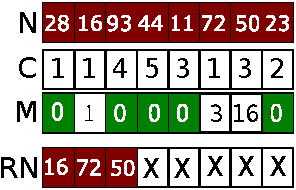
\includegraphics[width=.24\linewidth, height=.15\linewidth]{figures/ONPL_Conflict.pdf}\label{fig:cd}}\hspace{.05\linewidth}
  \subfigure[Code snippet to calculate mask M. \textit{pnt$\_$outEdges} represents the list of out edges, \textit{self$\_$loop$\_$mask} is the mask to prevent the self-loop and \textit{zeta} represents the list of community.]{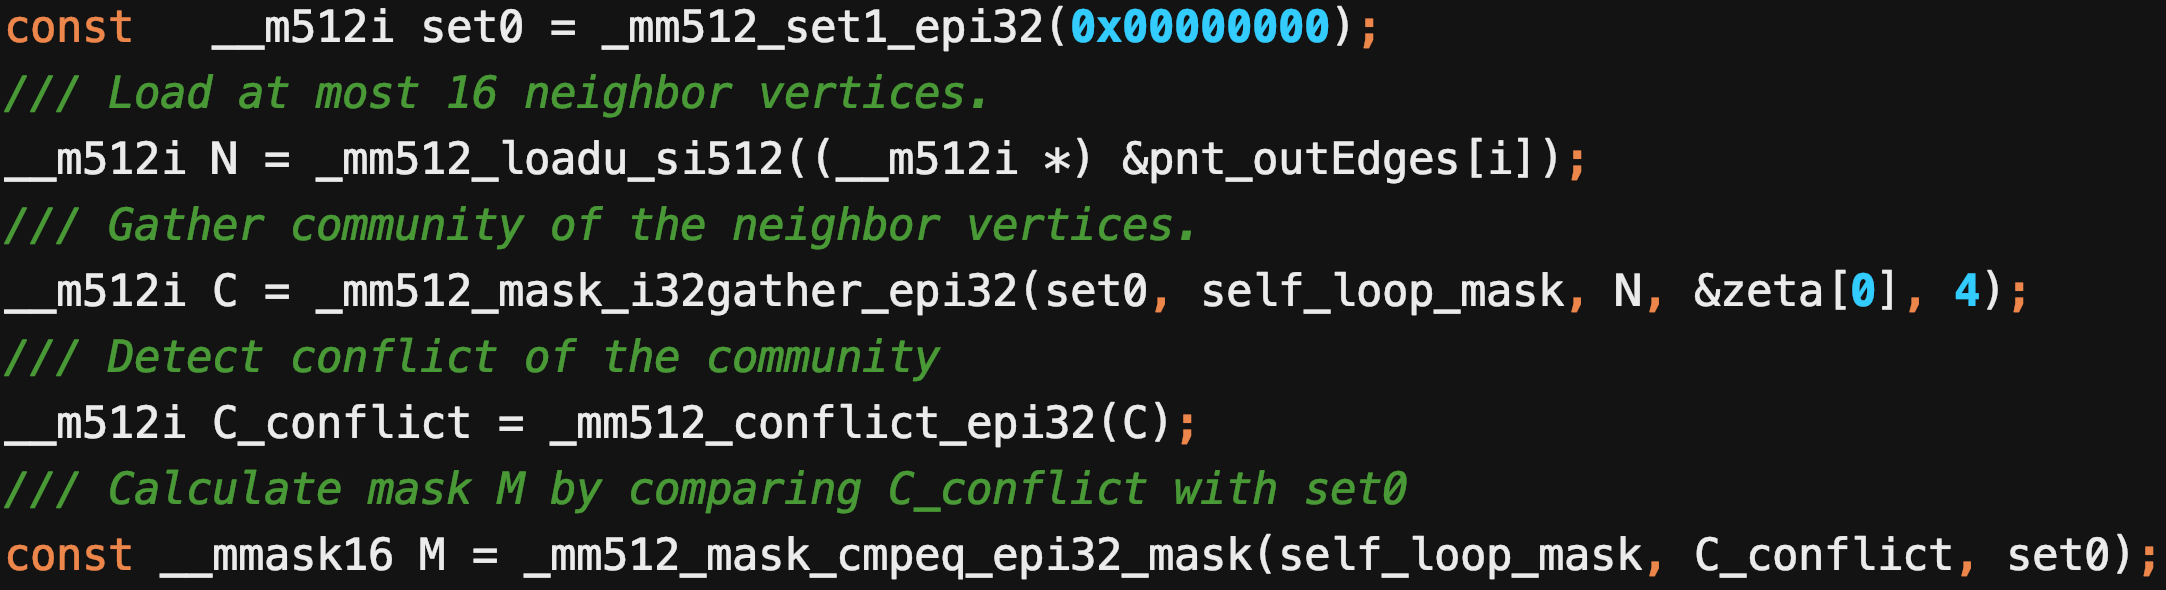
\includegraphics[width=.48\linewidth, height=.15\linewidth]{code/calculation_M_using_conflict.png}\label{fig:cd_code}}
  \caption{Perform reduce scatter using conflict detection. The neighbors (N) are  in their Communities (C). A mask (M) is derived from C 
  to denote the entries that will be processed (in green). Some neighbors will remain (RN) to be processed.
%  Two ways to perform reduce and scatter. The neighbors (N) are  in their Communities (C). A mask (M) is derived to denote the 
 % entries that will be processed (in green). Some neighbors will remain (RN) to be processed.
 }
  \label{fig:onpl_vector_lane_conflict}
\end{figure}
This instruction(\texttt{\_mm512\_conflict\_epi32} ) is the basis of the \textit{conflict detection} method for reduce and scatter as it enables the 
extraction of different sets of communities and neighbors that can safely process at the same time. Figure~\ref{fig:cd} represents the process. 
Here, \textit{N} is the list of neighbors of a vertex, and \textit{C} is the corresponding list of communities. 
Instruction(\texttt{\_mm512\_conflict\_epi32} ) is applied on \textit{C} to calculate the mask M. Figure~\ref{fig:cd_code} shows the code snippet 
to calculate the mask \textit{M}. 
There are two techniques to handle the conflicted case: the first iteratively performs the vector operation on the non-conflicted sets and performs 
as many iterations of vector operations as there are non-conflicted sets; the second one applies vector operation on a non-conflicted 
set of neighbors only once and performs the  remaining entries using purely scalar operations. Indeed, in practice, this conflict detection 
method uses many instructions. And it only useful if many communities can process at once. The vector will process one entry at 
a time with expensive vector operations if adjacent vertices belong to the same community. One can avoid the problem by performing 
vector operation only on the first set of independent communities and use the scalar operations afterward in the conflict detection method.

\begin{figure}[t]
  \centering
  \subfigure[In-vector Reduction.]{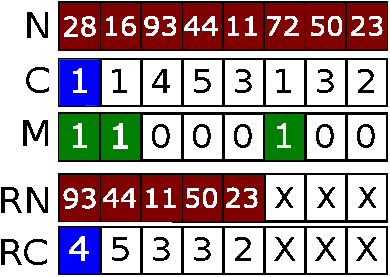
\includegraphics[width=.20\linewidth, height=.22\linewidth]{figures/ONPL_Compress.pdf}\label{fig:ivr}}\hspace{.05\linewidth}
  \subfigure[Code snippet to calculate mask M. \textit{pnt$\_$outEdges} represents the list of out edges, \textit{self$\_$loop$\_$mask} is the mask to prevent the self-loop and \textit{zeta} represents the list of community.]{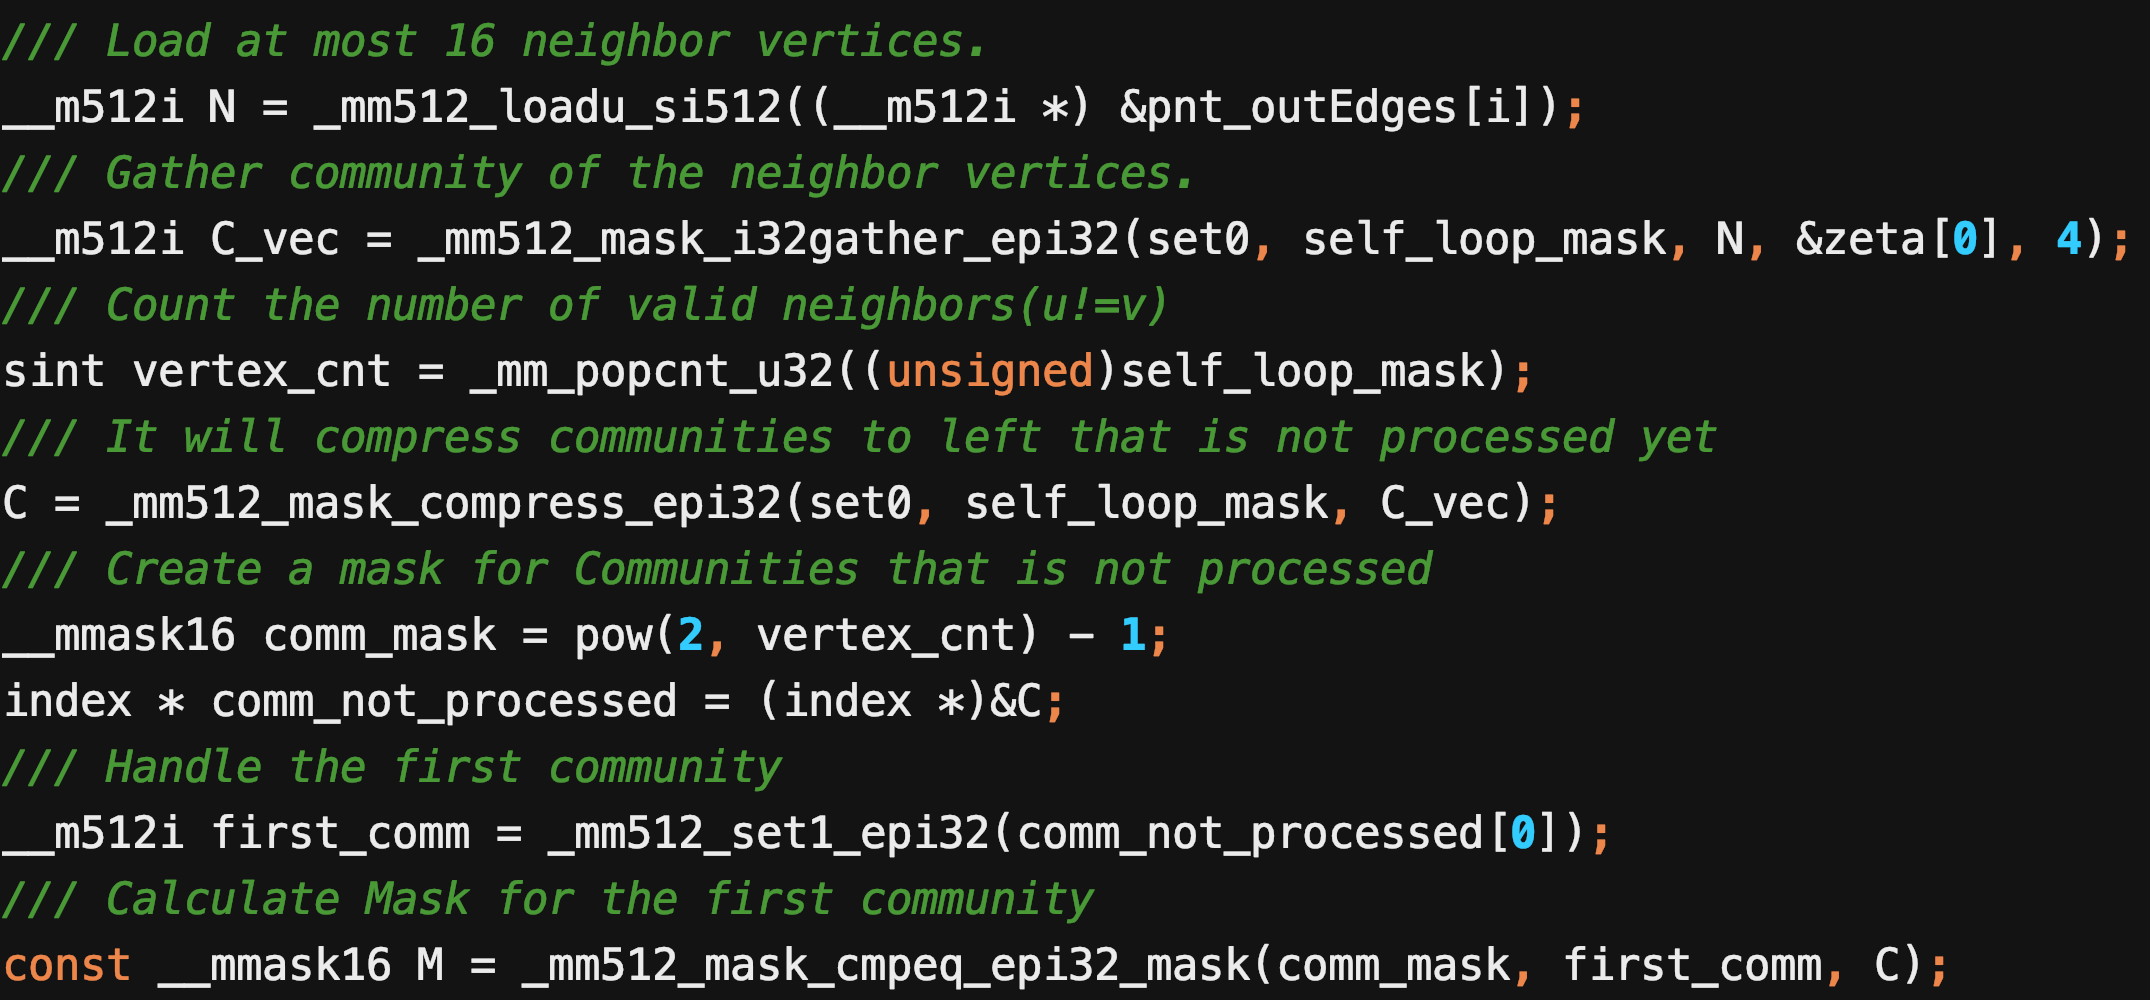
\includegraphics[width=.48\linewidth, height=.22\linewidth]{code/calculation_M_using_compressed.png}\label{fig:ivr_code}}
  \caption{
  Perform reduce scatter by compressing the communities. The neighbors (N) are  in their Communities (C). A mask (M) is derived from C 
  to denote the entries that will be processed (in green). Some neighbors(RN) and communities(RC) will remain to be processed.
  %Two ways to perform reduce and scatter. The neighbors (N) are in their Communities (C). A mask (M) is derived to denote the
%    entries that will be processed (in green). Some neighbors will remain (RN) to be processed.
    }
  \label{fig:onpl_vector_lane_compressed}
\end{figure}
Another extreme case comes when all the communities in the vector are identical. This case arises when the process has mostly converged. 
In this case, an \textit{in-vector reduction} is preferable. This method (sketched in Figure~\ref{fig:ivr}) masks out all the entries of the vector 
besides the one mapping to a particular community. Figure~\ref{fig:ivr_code} shows the code snippet to calculate the mask \textit{M}.
Then the edge weight mapping to this community is reduced with a masked reduction 
instruction \texttt{\_mm512\_mask\_reduce\_add\_ps} and is finally added back to the affinity of that community. 
In Figure~\ref{fig:ivr}, \textit{RN} represents the remaining vertices that are not processed yet, 
and \textit{RC} is the list of their corresponding communities. 
Similar to the conflict detection method, there are two ways to proceed. Successive communities can use mask 
and reduce; however, this can lead to an issue for vertices that sit at the border of many communities causing potentially a 
large vector overhead. In practice, ONPL only processes vector operations for the first community of the vector and defaults to 
scalar implementation for the remaining communities.

The calculation of modularity from the affinity and the assignment of vertices to the community is done with simple vector processing and 
does not pose particular challenges.

\subsection{ONLP: One Neighbor Per Lane Label Propagation}
Nodes traverse in a parallel fashion, which brings the randomization on the node selection. For each node, 
it loads 16 neighbors and gathers their corresponding labels at once. For each distinct label, it sums the 
neighbor edge weight to create a vector with label weight. Each vector lane handles one neighbor of the 
vertex. Then an Intrinsic instruction \textit{$\_mm512\_reduce\_max\_ps$} applied to find out the heaviest neighbor label. 
A vertex participates in the next iteration if any of its neighbor labels change.


\section{OVPL: One Vertex Per Lane}
\label{sec:ovpl}
In the One Vertex Per Lane (OVPL) method, each SIMD lane processes different vertices. 
%The vertices of the graph will be grouped in blocks so that the block size is a multiple of the number of lanes in the vector. 
Initially, vertices of the graph are group into multiple blocks where the size of blocks is the multiple of the vector lanes.
We have to restructure the network for the efficiency and convergence of the algorithm.

Because two vertices in a block will be processed simultaneously, OVPL requires two vertices in the same block 
not to be neighbors. Reordering the graph to have that property requires solving a graph coloring problem. 
Therefore it makes no sense to deploy OVPL for graph coloring. We only consider OVPL for the community detection problem.
\subsection{Preprocessing}
Vertices that are part of the same block will always be processed simultaneously. This property might induce race conditions 
that can prevent convergence. If the adjacent vertices are processed simultaneously, the affinity calculation performs on the 
changing information. The simplest case is a graph with two vertices that swaps their community infinitely, but the issue also 
appears on numerous complex networks.

To prevent this from happening, we first solve a graph coloring problem: we allocate a color to each vertex so 
that no two adjacent vertices have the same color. We then group the vertices where each group holds vertices 
with the same color. That will make sure that no vertices are adjacent in a group. While finding the coloring 
with a minimal number of colors is an NP-Complete problem~\cite{GareyJohnson79}, we do not require such a
high-quality solution. We use the speculative parallel greedy graph coloring
algorithm~\cite{Catalyurek12-ParCo} we described in Section~\ref{sec:pb-coloring}. 

After grouping the vertices, we sort the vertices in each group by non-increasing degrees. 
Sorting will help to minimize wasted computation during execution.

Finally, we split each group of non-adjacent vertices into small blocks of equal size equal to a multiple of 
the number of lanes. We reformat the vertices of each block to enable vectorization by interleaving the 
representation of the different vertices. That also reduces unaligned memory accesses. The format is similar to 
sliced ELLPACK~\cite{monakov2010automatically}. A contiguous memory of size $max\_deg\_of\_block$ $\times$ $block\_size$ 
holds each block of vertices. The index from $(i-1)$ $\times$ $block\_size$ to $i$ $\times$ $block\_size$ will 
represent the $i^{th}$ neighbor of the vertices of each block. Edge weights also follow a similar representation.

Figure~\ref{fig:graph_ovpl_preprocess} shows a sample graph and its block structure. In the example, we assume 
the vector length is 4 for readability (instead of 16). So, the initial block will hold vertices that are not 
adjacent by selecting the same color. But in the second group, there are no four vertices with the same color; 
that is why it contains vertices of different colors to fill the vector.
\begin{figure}[hbt]
  \centering
  \subfigure[Sample Graph]{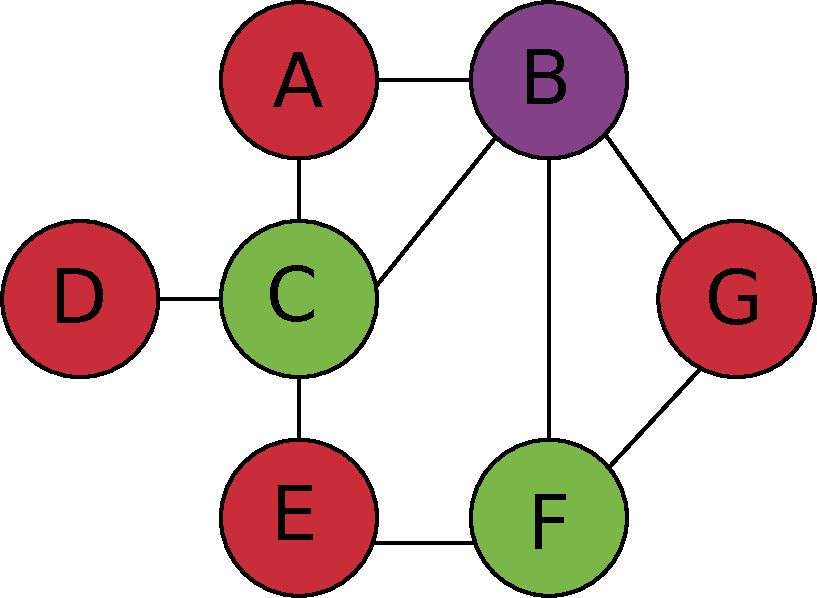
\includegraphics[width=.20\linewidth]{figures/sample_graph.pdf}}\hspace{.05\linewidth}
  \subfigure[Abstract Memory Representation]{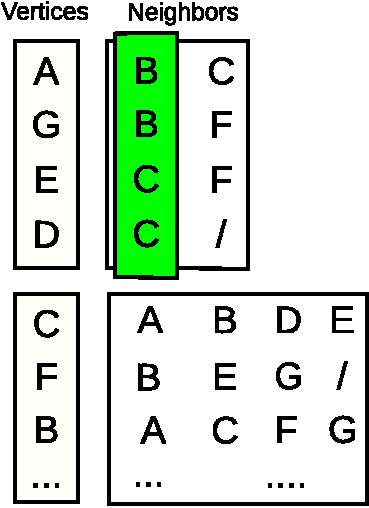
\includegraphics[width=.16\linewidth]{figures/OVPL_Preprocess.pdf} \xspace\xspace\xspace\xspace\xspace\xspace\xspace\xspace\xspace\xspace\xspace\xspace\xspace\xspace\xspace\xspace\xspace\xspace} %putting \xspace to unwrap the caption
  \subfigure[Physical Memory Representation]{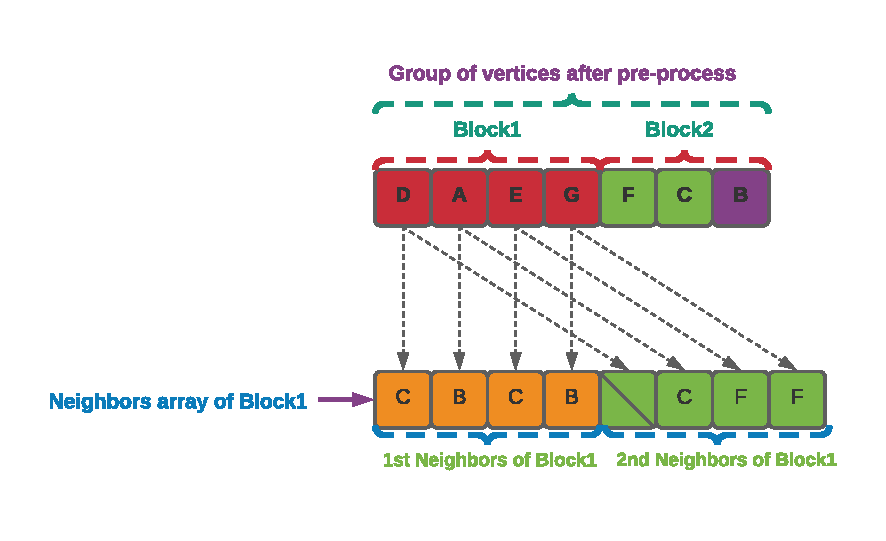
\includegraphics[width=.35\linewidth]{figures/ovpl_physical_memory.pdf}}
 
  \caption{OVPL reorders the graph using a graph coloring methods and
    structure it in blocks of vertices so that the neighbors of the
    vertices of a block can be loaded in a vector (sketched in green)
    simultaneously.}
  \label{fig:graph_ovpl_preprocess}
\end{figure}

\subsection{Moving a Block of Vertices}
Rather than moving a vertex to its most preferable community, OVPL \textit{moves} a block of vertices at once. It calculates 
the \textit{affinity} of all the vertices of a block concurrently. Therefore OVPL has a much higher memory utilization than 
PLM because it keeps $block\_size$ affinity structures in memory.

OVPL computes the affinity of each vertex of the block one neighbor at
a time. OVPL first loads the first neighbor of each vertex of the
block at once and gathers the community of the first neighbors. Then it
gathers the affinity of the neighbor communities from the different
affinity arrays. OVPL adds the edge weights to the obtained affinity
and scatters the updated values back to the appropriate locations. Note that because of this, 
it was not possible to perform this vectorization on x86 processors before scatter was introduced with AVX-512.

This process repeats until all the neighbors of all the vertices of the block are processed, i.e., until the maximum 
degree of the block. However, some vertices may have a lower degree, so OVPL needs to check the existence of the 
neighbor. This check increases the number of instructions and causes the algorithm to use masked vector instructions. 
OVPL does not perform that check before the minimum degree of the block neighbors has been considered. 
The difference between the maximum and minimum degree in each block leads to wasted SIMD lanes. Preprocessing 
sorted the different color groups per degree to minimize the degree difference. 
Also representing the blocks by interleaving the vertices, enables access to the graph to aligned loads.

The assignment of vertices to new communities is done without
particular optimization using a natural way of performing this task.


\section{Experimental Settings}
\label{sec:expsetting}
\paragraph{Hardware Platform and Operating System.}
We used two different machines for the two architectures we study in this paper. 
We refer to the first machine as \texttt{SkylakeX}. It is a node with two 
Intel Xeon Gold 6154 processors (SkylakeX architecture, 18 cores per processor, no hyperthreading, 25MB L3 Cache) and 388 GB of DDR4 memory. 
The second machine is \texttt{Cascade Lake}, which is equipped with two Intel Xeon Gold model 6248R (Cascade Lake architecture, 
24 cores per processor, no hyperthreading, 36MB L3 Cache) and 384GB GB of DDR4 memory. Both processors support Intel \texttt{AVX-512F} 
and \texttt{AVX-512CD} instruction sets with among others. Both machines use Linux \texttt{3.10.0}. 

\paragraph{Software Environment.}
All the codes are compiled by the Intel C++ compiler \texttt{icpc} version \texttt{16.0.0.109}. Codes also compile 
with optimization flag \texttt{-O3} and \texttt{xCORE-AVX512} flags, so the compiler generates a binary optimized  for the architecture. 
We pick existing established code bases for both algorithms to confirm we start from implementations of reasonable good qualities.

We build graph coloring and community detection experiments on top of Kokkos~\cite{edwards2014kokkos} and 
\textit{NetworKit}~\cite{staudt2014networkit}, respectively. We intended to compare to the original PLM implementation
from~\cite{plm}.  During our experiments, we realized that PLM suffered from various memory management issues like 
large buffers were allocated and deallocated for each vertex traversed. We created a Modified PLM implementation (MPLM) 
that preallocates memory per thread. And then reuse the same buffer for the computation rather than deallocating and 
reallocating memory over and over. After confirming that MPLM is an improvement on PLM (See section~\ref{sec:mplm:compare}), 
we will perform all other comparisons with MPLM.


\paragraph{Graphs.}
We perform our experiments on real-world data sets to avoid the
bias introduced by random graph generator.
We select graphs from the \textit{Stanford Large Network Dataset Collection} 
(SNAP)~\cite{snapnets} and \textit{DIMACS}~\cite{sanders2014benchmarking,bader2013graph} data sets that are well known 
for graph algorithm research. Graphs are from different categories like Social networks, clustering instances, sparse matrices, 
internet topology networks, citation networks. We expect that the coverage in the type of graphs 
enables deriving conclusions that are more general and bias-free than picking all graphs from a single category. 
\\
Table~\ref{tab:Graphlist}  presents the list of undirected graphs that we use in the experiments. The table also includes 
basic statistics such as the number of nodes ($V$), edges ($E$) of the graph, the maximum degree of the graph ($\Delta$), 
and average degree ($\delta$).
\\
\begin{table}[htb]
 % \small
\caption{List of graphs used in the experiment}
\label{tab:Graphlist}
\centering
\begin{tabular}[c]{| l | r | r | r | r |}
\hline
Graph & Nodes ($V$) & Edges ($E$) & $\Delta$ & $\delta$ \\ \hline
333SP  &  3,712,815  &  11,108,633  &  28  &  5  \\ \hline
AS365  &  3,799,275  &  11,368,076  &  14  &  5  \\ \hline
M6  &  3,501,776  &  10,501,936  &  10  &  5  \\ \hline
NACA0015  &  1,039,183  &  3,114,818  &  10  &  5  \\ \hline
NLR  &  4,163,763  &  12,487,976  &  20  &  5  \\ \hline
Oregon-2  &  11,806  &  32,730  &  2,432  &  5  \\ \hline
asia  &  11,950,757  &  12,711,603  &  9  &  2  \\ \hline
belgium  &  1,441,295  &  1,549,970  &  10  &  2  \\ \hline
delaunay$\_$n24  &  16,777,216  &  50,331,601  &  26  &  5  \\ \hline
europe  &  50,912,018  &  54,054,660  &  13  &  2  \\ \hline
germany  &  11,548,845  &  12,369,181  &  13  &  2  \\ \hline
in-2004  &  1,382,908  &  13,591,473  &  21,869  &  19  \\ \hline
kkt$\_$power  &  2,063,494  &  6,482,320  &  95  &  6  \\ \hline
loc-Gowalla  &  196,591  & 950,327 & 14,730 & 9  \\ \hline
luxembourg  &  114,599  &  119,666  &  6  &  2  \\ \hline
netherlands  &  2,216,688  &  2,441,238  &  7  &  2  \\ \hline
nlpkkt200  &  16,240,000  &  215,992,816  &  27  &  26  \\ \hline
roadNet-PA  &  1,088,092  &  1,541,898  &  9  &  2  \\ \hline
uk-2002  &  18,520,486  &  261,787,258  &  194,955  &  28  \\ \hline
\end{tabular}
\end{table}


\paragraph{Collection of Result Sets.}
All the variants are run 25 times for each graph. The reported values
of time and modularity are average of the 25 runs. For
runtime, we only measure the time taken by the community detection(\textit{Move-Phase}) and graph coloring 
algorithm itself, not the time spent reading the graph from the
file system. We computed the 95\% \textit{confidence interval}~\cite{efron1986bootstrap} for the results of all the
experiments. Once we realized  the confidence intervals were very narrow and that the visible differences in the plots were statistically 
significant, we choose not to report them to improve figures readability.

%% The experiment results of the benchmark set the expectation for our problems. For a graph with a large degree and the best diagonal 
%% layout, SkylakeX is only 10\% faster using vector instructions than scalar ones. Meanwhile, KNL should see performance improvement, 
%% up to a factor of 3.5 on graphs with moderately high degrees. Practically, the performance improvement brought by vectorization will 
%% be lower, especially since we will be reporting application performance and not kernel performance.

\section{Performance Results}
\subsection{Microbenchmark}

The microbenchmark simulates the affinity calculation of a single
vertex in a fairly dense graph (with 4096 neighbors per-vertex packed
along the diagonal). The code does a sequence similar to the
operations of the algorithms we consider: load, gather, and
scatter when running vectorially. The benchmark is written to
compare a scalar implementation and a vector implementation.

\begin{figure}[!bt]
  \centering
  %\subfigure[KNL]{\includegraphics[page=21,width=.48\linewidth]{ubenchplots/benchmark_KNL.pdf}}
  %
%  \subfigure[SkylakeX]{
  \includegraphics[page=20,width=.48\linewidth]{ubenchplots/benchmark_SkylakeX.pdf}
  
  \caption{Microbenchmark performance on SkylakeX.}
  \label{fig:microbench}
\end{figure}

The results for the SkylakeX architectures (in Figure~\ref{fig:microbench})
highlight that there are little differences in SkylakeX between
the scalar and vectorized performance, with the vector implementation
being 20\% faster than the scalar one. 

This sets the expectation for our problems. The microbenchmark is
essentially what graph coloring does. For a graph with a large degree
and the best diagonal layout, SkylakeX is only 20\% faster using
vector instructions than scalar ones. The community detection problem 
could see higher improvements because the 
problem is more computational.


\begin{figure}[t]
  \centering
 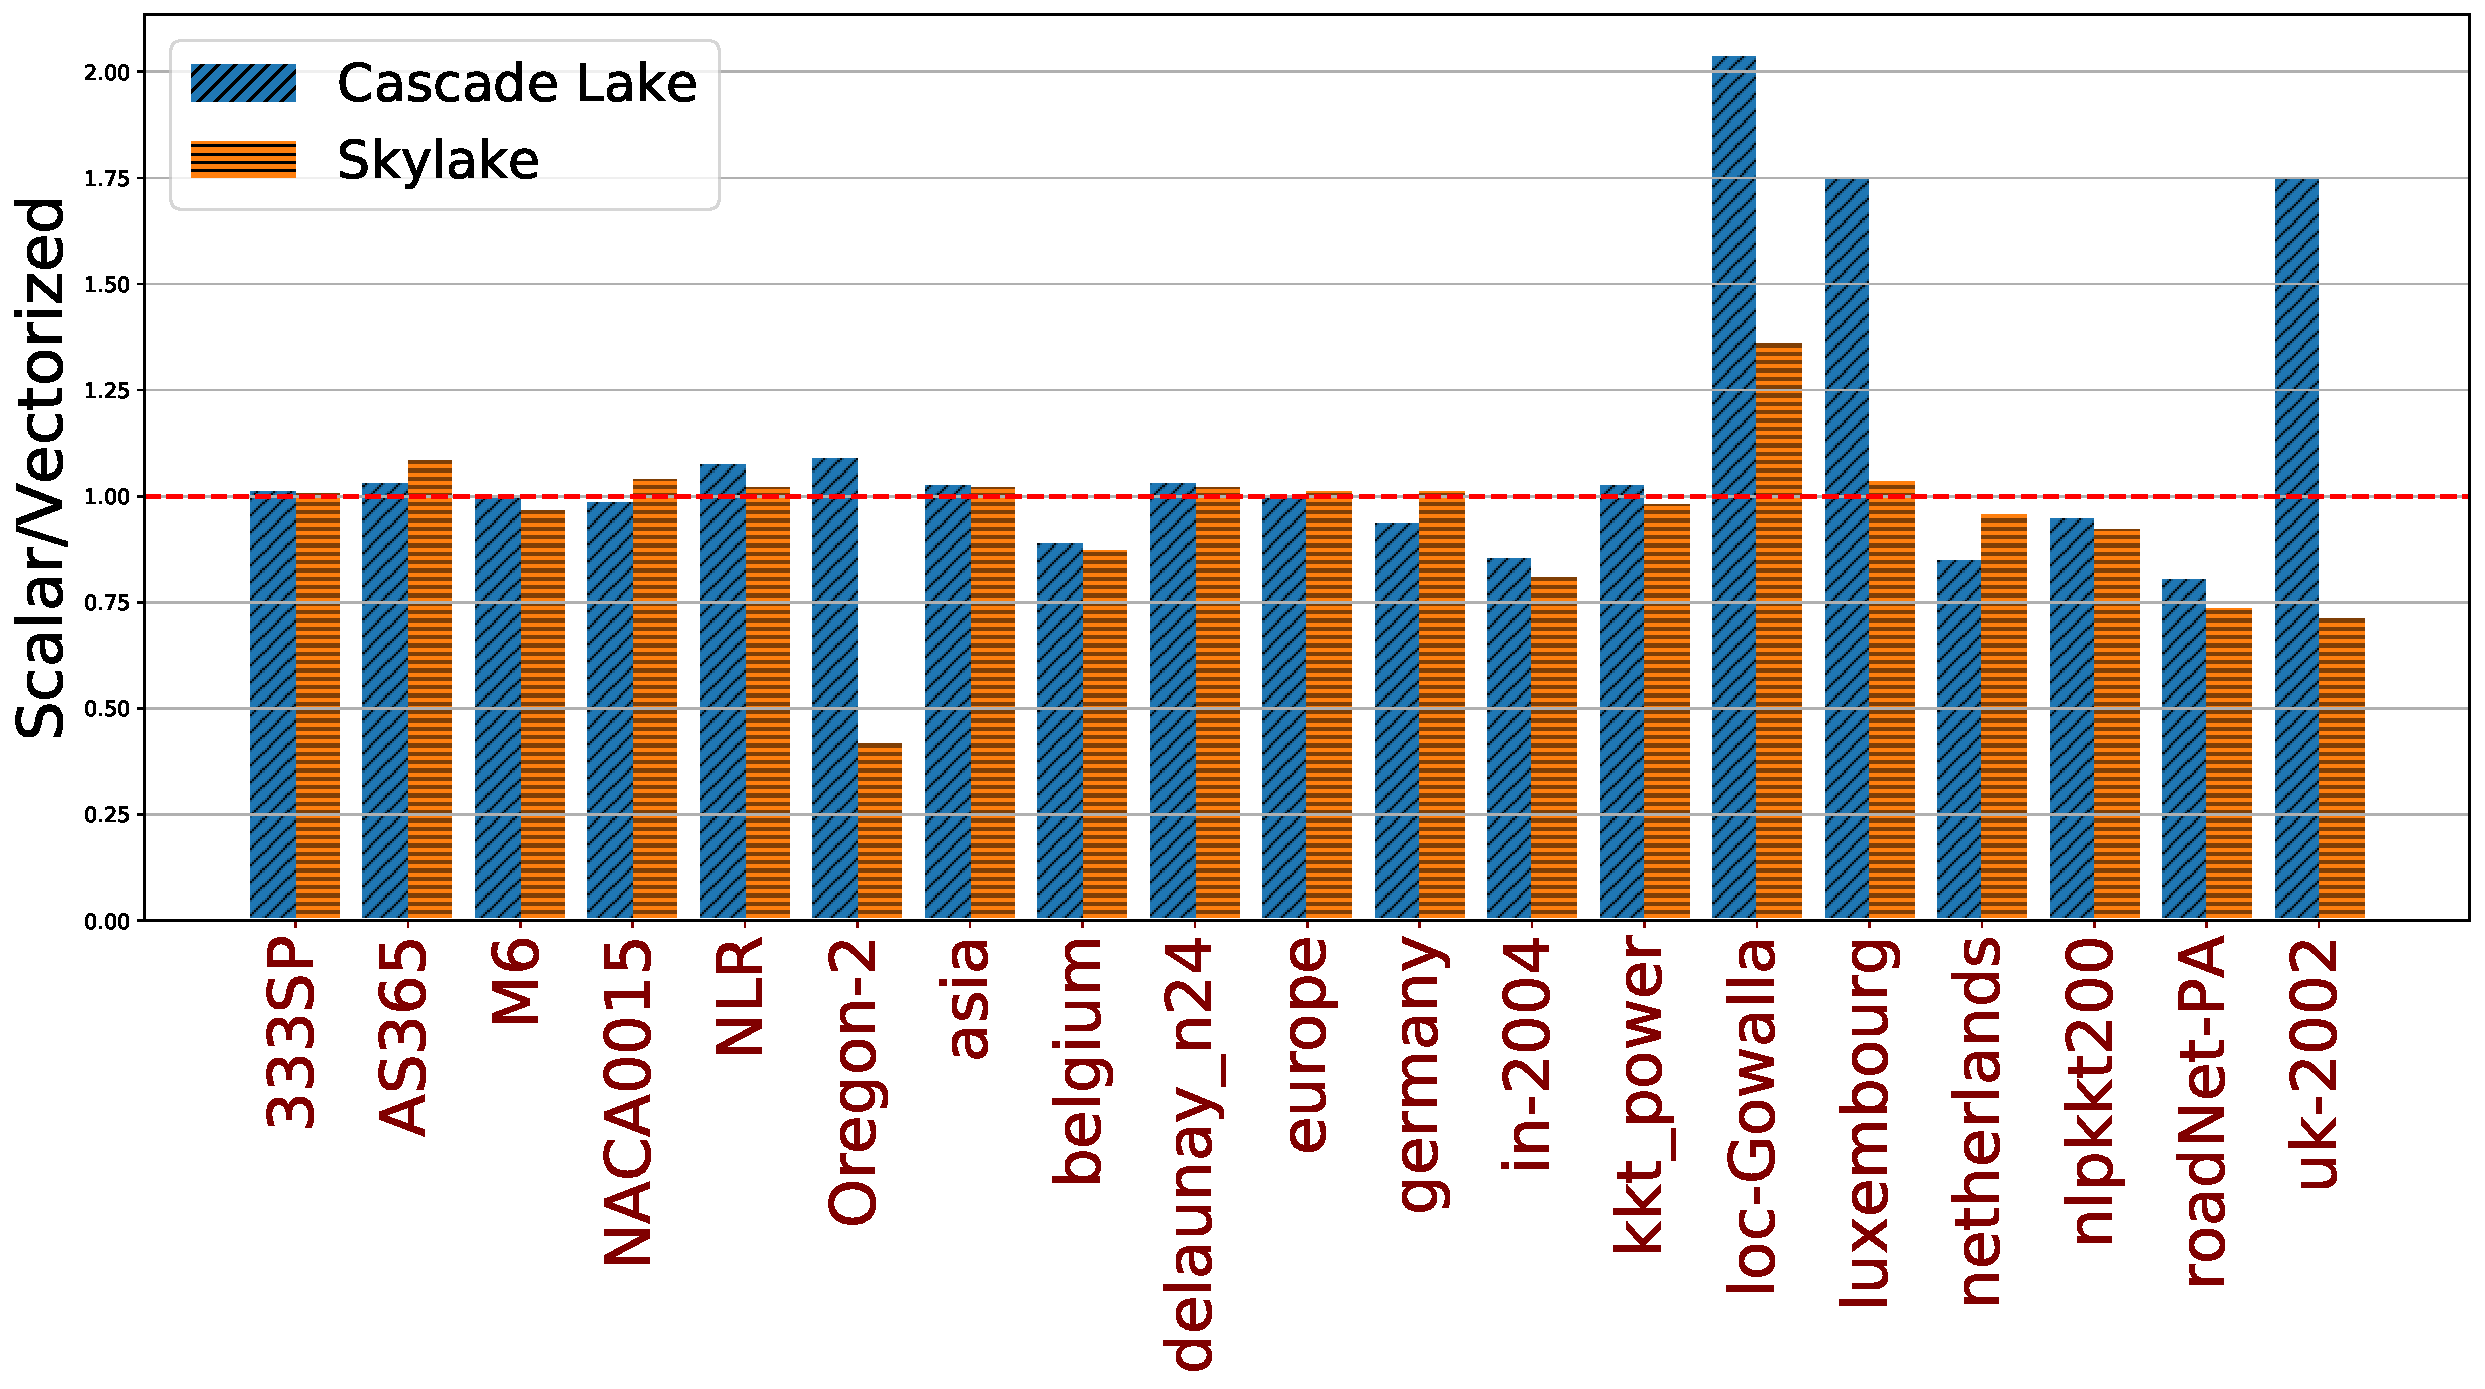
\includegraphics[width=.48\linewidth]{figures/coloring/coloring_scalar_vs_vec_threads_cascade_48_skl_36.pdf}    
  \caption{[Graph Coloring] Impact of vectorization of Graph Coloring on both architectures. Y-axis represents the normalized version of 
  the runtime comparison between scalar and vectorized. Scalar/Vectorized = 2.5 means vectorized version is 2 
  times faster than scalar.}
   \label{fig:coloring_cascade_48_skl_36}
\end{figure}

\label{sec:perf}
\subsection{Speculative Greedy Graph Coloring}
The performance of the ONPL vectorization on graph coloring is displayed in Figure~\ref{fig:coloring_cascade_48_skl_36} 
for the \textit{Cascade Lake} and \textit{SkylakeX} architectures. Vectorized speculative graph coloring on both processors 
shows moderate performance enhancement for some graphs over the scalar version. Vectorized graph coloring on the 
Cascade Lake and SkylakeX outperform the scalar version by at most factors of $2$ and $1.4$. Speculative parallel graph coloring 
has two main parts. One is the assignment of color, and another is conflict detection. We only apply vectorization on the 
color assignment portion. Graph coloring has a limited opportunity for vectorization that is why it shows a moderate 
performance for most of the graphs. 

\subsection{Performance on R-MAT Graph}
\label{sec:rmat}
\subsubsection{R-MAT Graph}
R-MAT~\cite{chakrabarti2004r} is one of the most common synthesis graph generators which aims to maintain 
the power law of the natural graph. To generate a graph using R-MAT, one usually 6 attributes. First one is the 
\textit{scale} which determine the number of nodes $(2^{scale})$ in the graph. Next attribute is the \textit{edge-factor} 
which maintain the average degree of the graph. Then 4 parameters (a, b, c, d) to maintain probability distribution 
of edges among nodes. Usually adjacency matrix divided into 4 quad and each edge choose one quad based on the 
probability of that quad. R-MAT graph useful to describe results based on the structure of the graph. Here is the list 
of parameters we used to generate R-MAT graphs and to make it fair we perform different version of Label Propagation 
and Louvain method on the same graph. Table~\ref{tab:rmat_graph} represents parameters we used to generate 
R-MAT graph. 
\begin{table*}[htb]
 % \small
\caption{R-MAT Parameters}
\label{tab:rmat_graph}
\centering
\begin{tabular}[c]{| l | r | l |}
\hline
Scale & Edge-factor & Probability Distribution\\ \hline
\multirow{3}{*}{17, 18, 19, 20, 21, 22, 23, 24} & \multirow{3}{*}{1, 2, 4, 8, 16, 32, 64, 128} & a=33\%, b=33\%, c=33\%, and d=1\% \\ \cline{3-3}
 &  & a=40\%, b=30\%, c=20\%, and d=10\% \\ \cline{3-3}
 &  & a=57\%, b=19\%, c=19\%, and d=5\% \\ \hline
\end{tabular}
\end{table*}

\subsubsection{Label Propagation}
\begin{figure*}[hbt]
  		\centering
	\subfigure[RMAT parameters a=33\%, b=33\%, c=33\%, and d=1\%]{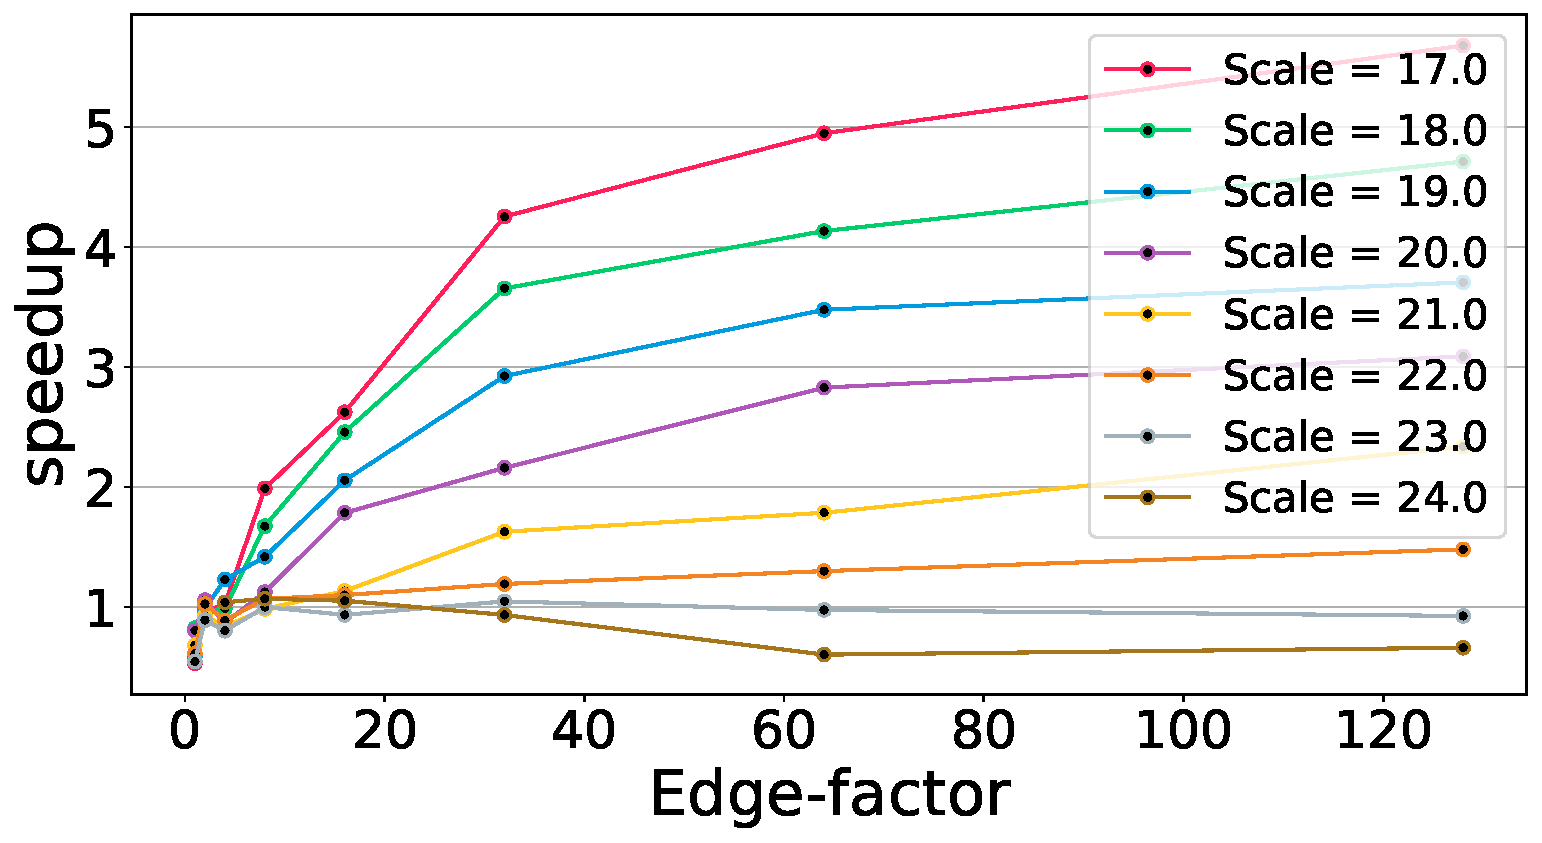
\includegraphics[page=1,width=.32\linewidth]{figures/rmat/cascade_label_propagation_perfomance_gain_against_edge_factor.pdf} \label{fig:rmat_lp_ef_1}}
	\subfigure[RMAT parameters a=40\%, b=30\%, c=20\%, and d=10\%]{\includegraphics[page=2,width=.32\linewidth]{figures/rmat/cascade_label_propagation_perfomance_gain_against_edge_factor.pdf} \label{fig:rmat_lp_ef_2}}
	\subfigure[RMAT parameters a=57\%, b=19\%, c=19\%, and d=5\%]{\includegraphics[page=3,width=.32\linewidth]{figures/rmat/cascade_label_propagation_perfomance_gain_against_edge_factor.pdf} \label{fig:rmat_lp_ef_3}}
	\caption{Performance gain of the ONPL Label propagation against scalar on the RMAT graph with different edge-factor on Cascade Lake processor.}
  \label{fig:rmat_lp_ef}
\end{figure*}
Figure~\ref{fig:rmat_lp_ef} and~\ref{fig:rmat_lp_nodes} shows the performance of the Label propagation on R-MAT graph on the 
Cascade Lake processor. We can see from Figure~\ref{fig:rmat_lp_ef} that performance gain of the Label propagation increased 
with higher edge-factor. Now, ONPL perform vectorization on one neighbor per lane that means higher edge-factor enable 
higher vectorization. We can also notice that performance of the application higher for the lower scale graph. Which gives the 
insight of the overall graph size has huge impact on the performance. Number of edges of a R-MAT calculated by 
$2^{scale}\times (2\times edge-factor)$.  Now, bigger graph brings higher cache misses because of the limitation of the memory size. 
So, if a graph shows higher average degree and size of the graph accommodate by the system memory then vectorized ONPL Label 
propagation will show a tremendous performance compare to scalar version. Figure~\ref{fig:rmat_lp_nodes} also provide 
similar evidence that smaller size (vertices) graph with higher edge-factor provide huge spike in performance gain.  

\begin{figure*}[hbt]
	\centering
	\subfigure[RMAT parameters a=33\%, b=33\%, c=33\%, and d=1\%]{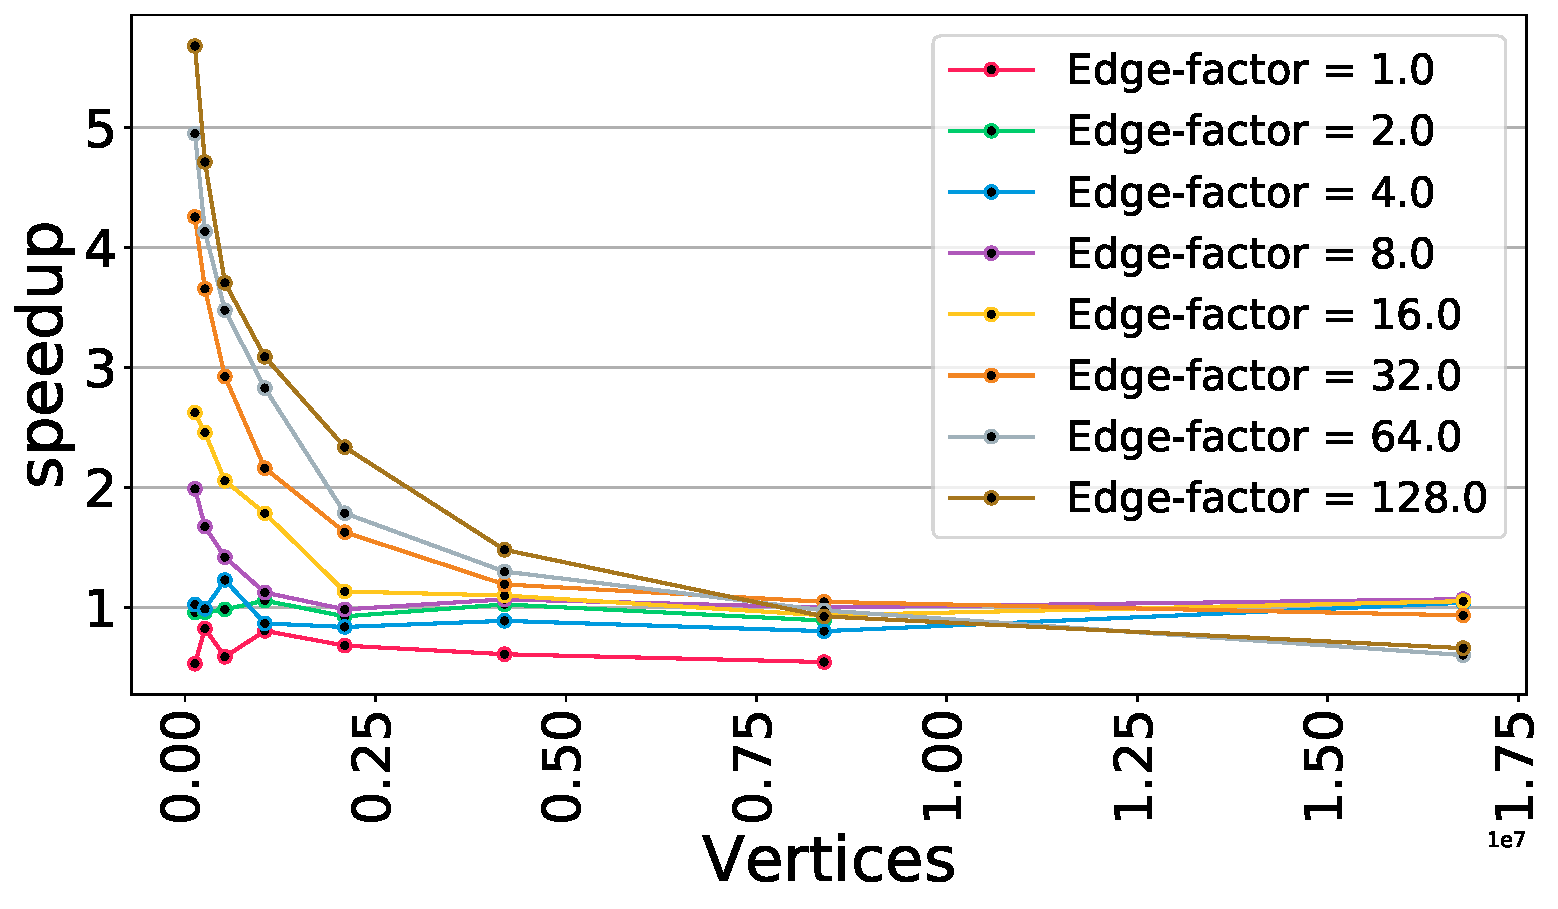
\includegraphics[page=1,width=.32\linewidth]{figures/rmat/cascade_label_propagation_perfomance_gain_against_vertices.pdf}\label{fig:rmat_lp_nodes_1}}
	\subfigure[RMAT parameters a=40\%, b=30\%, c=20\%, and d=10\%]{\includegraphics[page=2,width=.32\linewidth]{figures/rmat/cascade_label_propagation_perfomance_gain_against_vertices.pdf}\label{fig:rmat_lp_nodes_2}}
	\subfigure[RMAT parameters a=57\%, b=19\%, c=19\%, and d=5\%]{\includegraphics[page=3,width=.32\linewidth]{figures/rmat/cascade_label_propagation_perfomance_gain_against_vertices.pdf}\label{fig:rmat_lp_nodes_3}}
	\caption{Performance gain of the ONPL Label propagation against scalar on the RMAT graph with different different number of vertices on Cascade Lake processor.}
  \label{fig:rmat_lp_nodes}
\end{figure*}

\subsubsection{Louvain Method}
Figure~\ref{fig:rmat_lv_ef} and~\ref{fig:rmat_lv_nodes} show the performance of the Louvain method on the R-MAT graph. Louvain method 
shows the similar nature but the performance gain lower than the Label Propagation. One of the main reasons, the calculation of the 
Louvain method way much complex than Label Propagation. Memory usages is also higher in Louvain method which led more cache 
misses. But experiments on the R-MAT graph follow the main argument of the work that one should choose vectorized version ONPL 
Label propagation and Louvain for graphs with higher averages edges. If a graph shows lower average degree then scalar version 
is well suitable.
\begin{figure*}[hbt]
 	\centering
  	\subfigure[RMAT parameters a=33\%, b=33\%, c=33\%, and d=1\%]{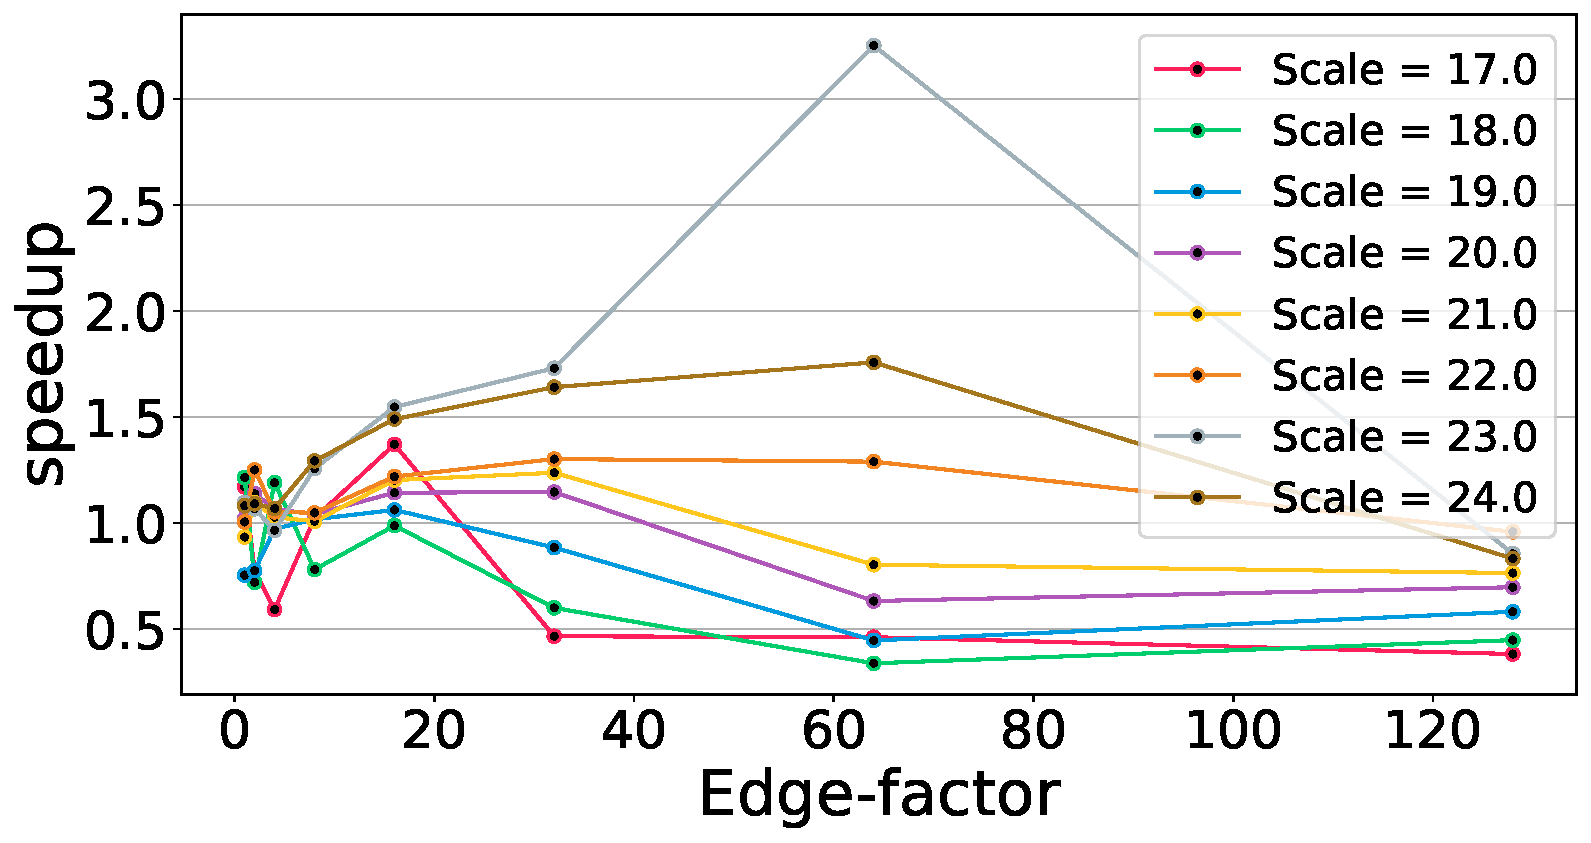
\includegraphics[page=1,width=.32\linewidth]{figures/rmat/cascade_onpl_perfomance_gain_against_edge_factor.pdf}\label{fig:rmat_lv_ef_1}}
  	\subfigure[RMAT parameters a=40\%, b=30\%, c=20\%, and d=10\%]{\includegraphics[page=2,width=.32\linewidth]{figures/rmat/cascade_onpl_perfomance_gain_against_edge_factor.pdf}\label{fig:rmat_lv_ef_2}}
  	\subfigure[RMAT parameters a=57\%, b=19\%, c=19\%, and d=5\%]{\includegraphics[page=3,width=.32\linewidth]{figures/rmat/cascade_onpl_perfomance_gain_against_edge_factor.pdf}\label{fig:rmat_lv_ef_3}}
	\caption{Performance gain of the ONPL Louvain Method against scalar on the RMAT graph with different edge-factor on Cascade Lake processor.}
  \label{fig:rmat_lv_ef}
\end{figure*}

\begin{figure*}[hbt]
	\centering
	\subfigure[RMAT parameters a=33\%, b=33\%, c=33\%, and d=1\%]{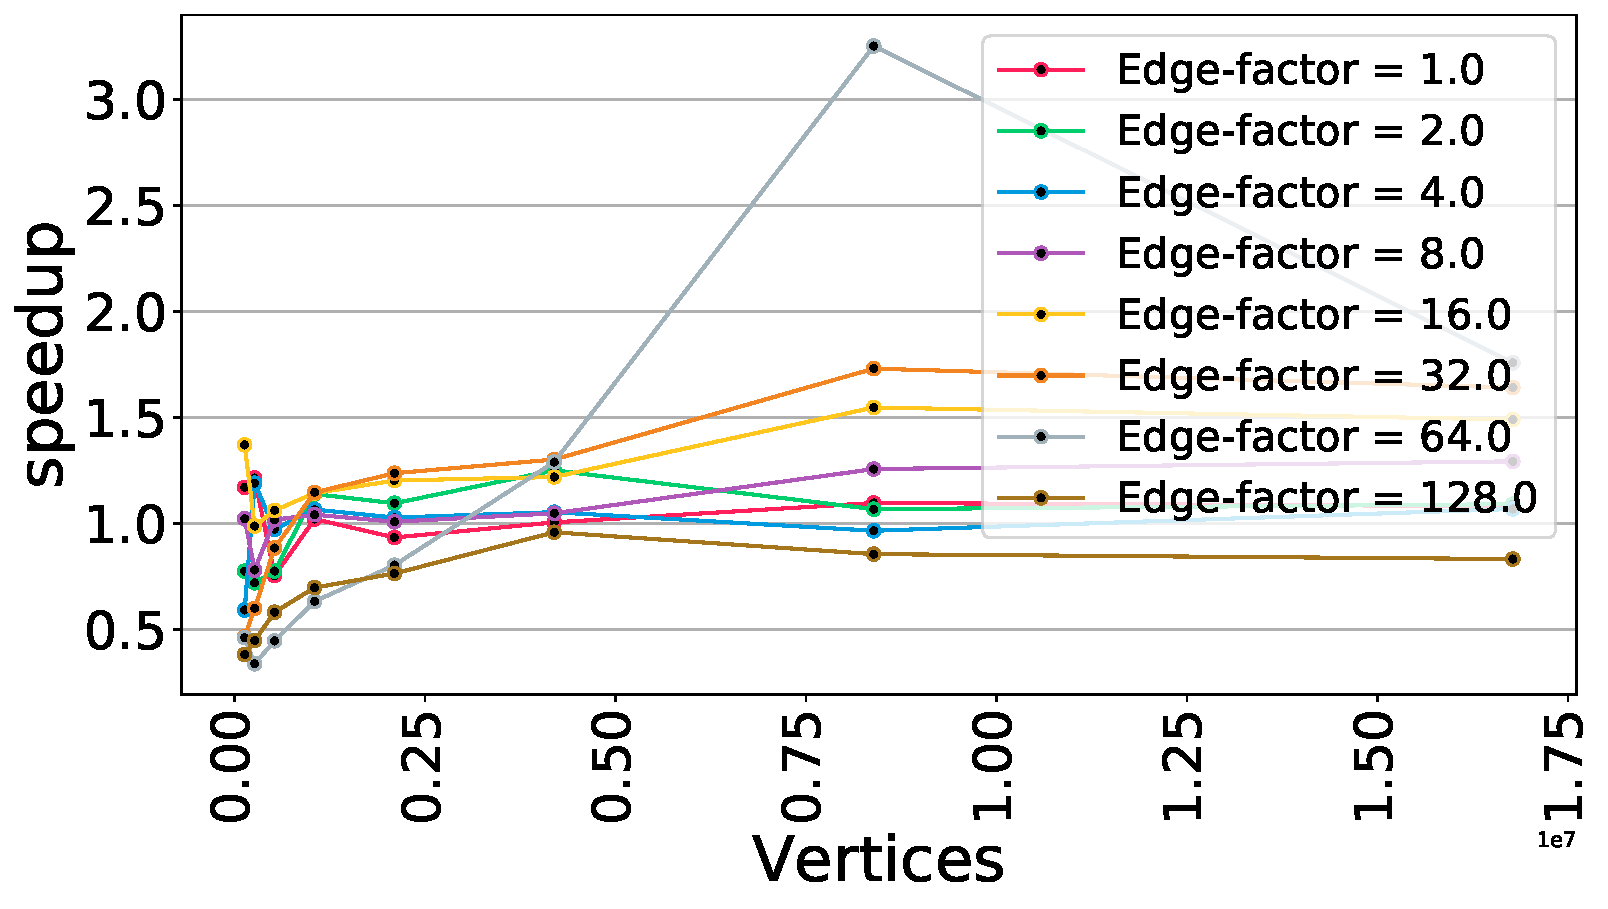
\includegraphics[page=1,width=.32\linewidth]{figures/rmat/cascade_onpl_perfomance_gain_against_vertices.pdf}\label{fig:rmat_lv_nodes_1}}
	\subfigure[RMAT parameters a=40\%, b=30\%, c=20\%, and d=10\%]{\includegraphics[page=2,width=.32\linewidth]{figures/rmat/cascade_onpl_perfomance_gain_against_vertices.pdf}\label{fig:rmat_lv_nodes_2}}
	\subfigure[RMAT parameters a=57\%, b=19\%, c=19\%, and d=5\%]{\includegraphics[page=3,width=.32\linewidth]{figures/rmat/cascade_onpl_perfomance_gain_against_vertices.pdf}\label{fig:rmat_lv_nodes_3}}
	\caption{Performance gain of the ONPL Louvain Method against scalar on the RMAT graph with different different number of vertices on Cascade Lake processor.}
  \label{fig:rmat_lv_nodes}
\end{figure*}


\subsection{Louvain Method on NetworKit}
\subsubsection{Modified Parallel Louvain Method (MPLM)}
\label{sec:mplm:compare}
We noticed some performance deficiencies in PLM, like threads reallocation of 
the memory needed for the affinity computation for each vertex that it encounters. To be able to study the impact of vector 
processing, we needed to make sure that the performance difference was rooted in vectorization rather than in memory 
management. The Modified Parallel Louvain Method (MPLM) is the code that contains various performance fixes for PLM.
\begin{figure*}[t]
	\centering
	\subfigure[PLM vs MPLM  speedup on the Cascade Lake(48 threads).]{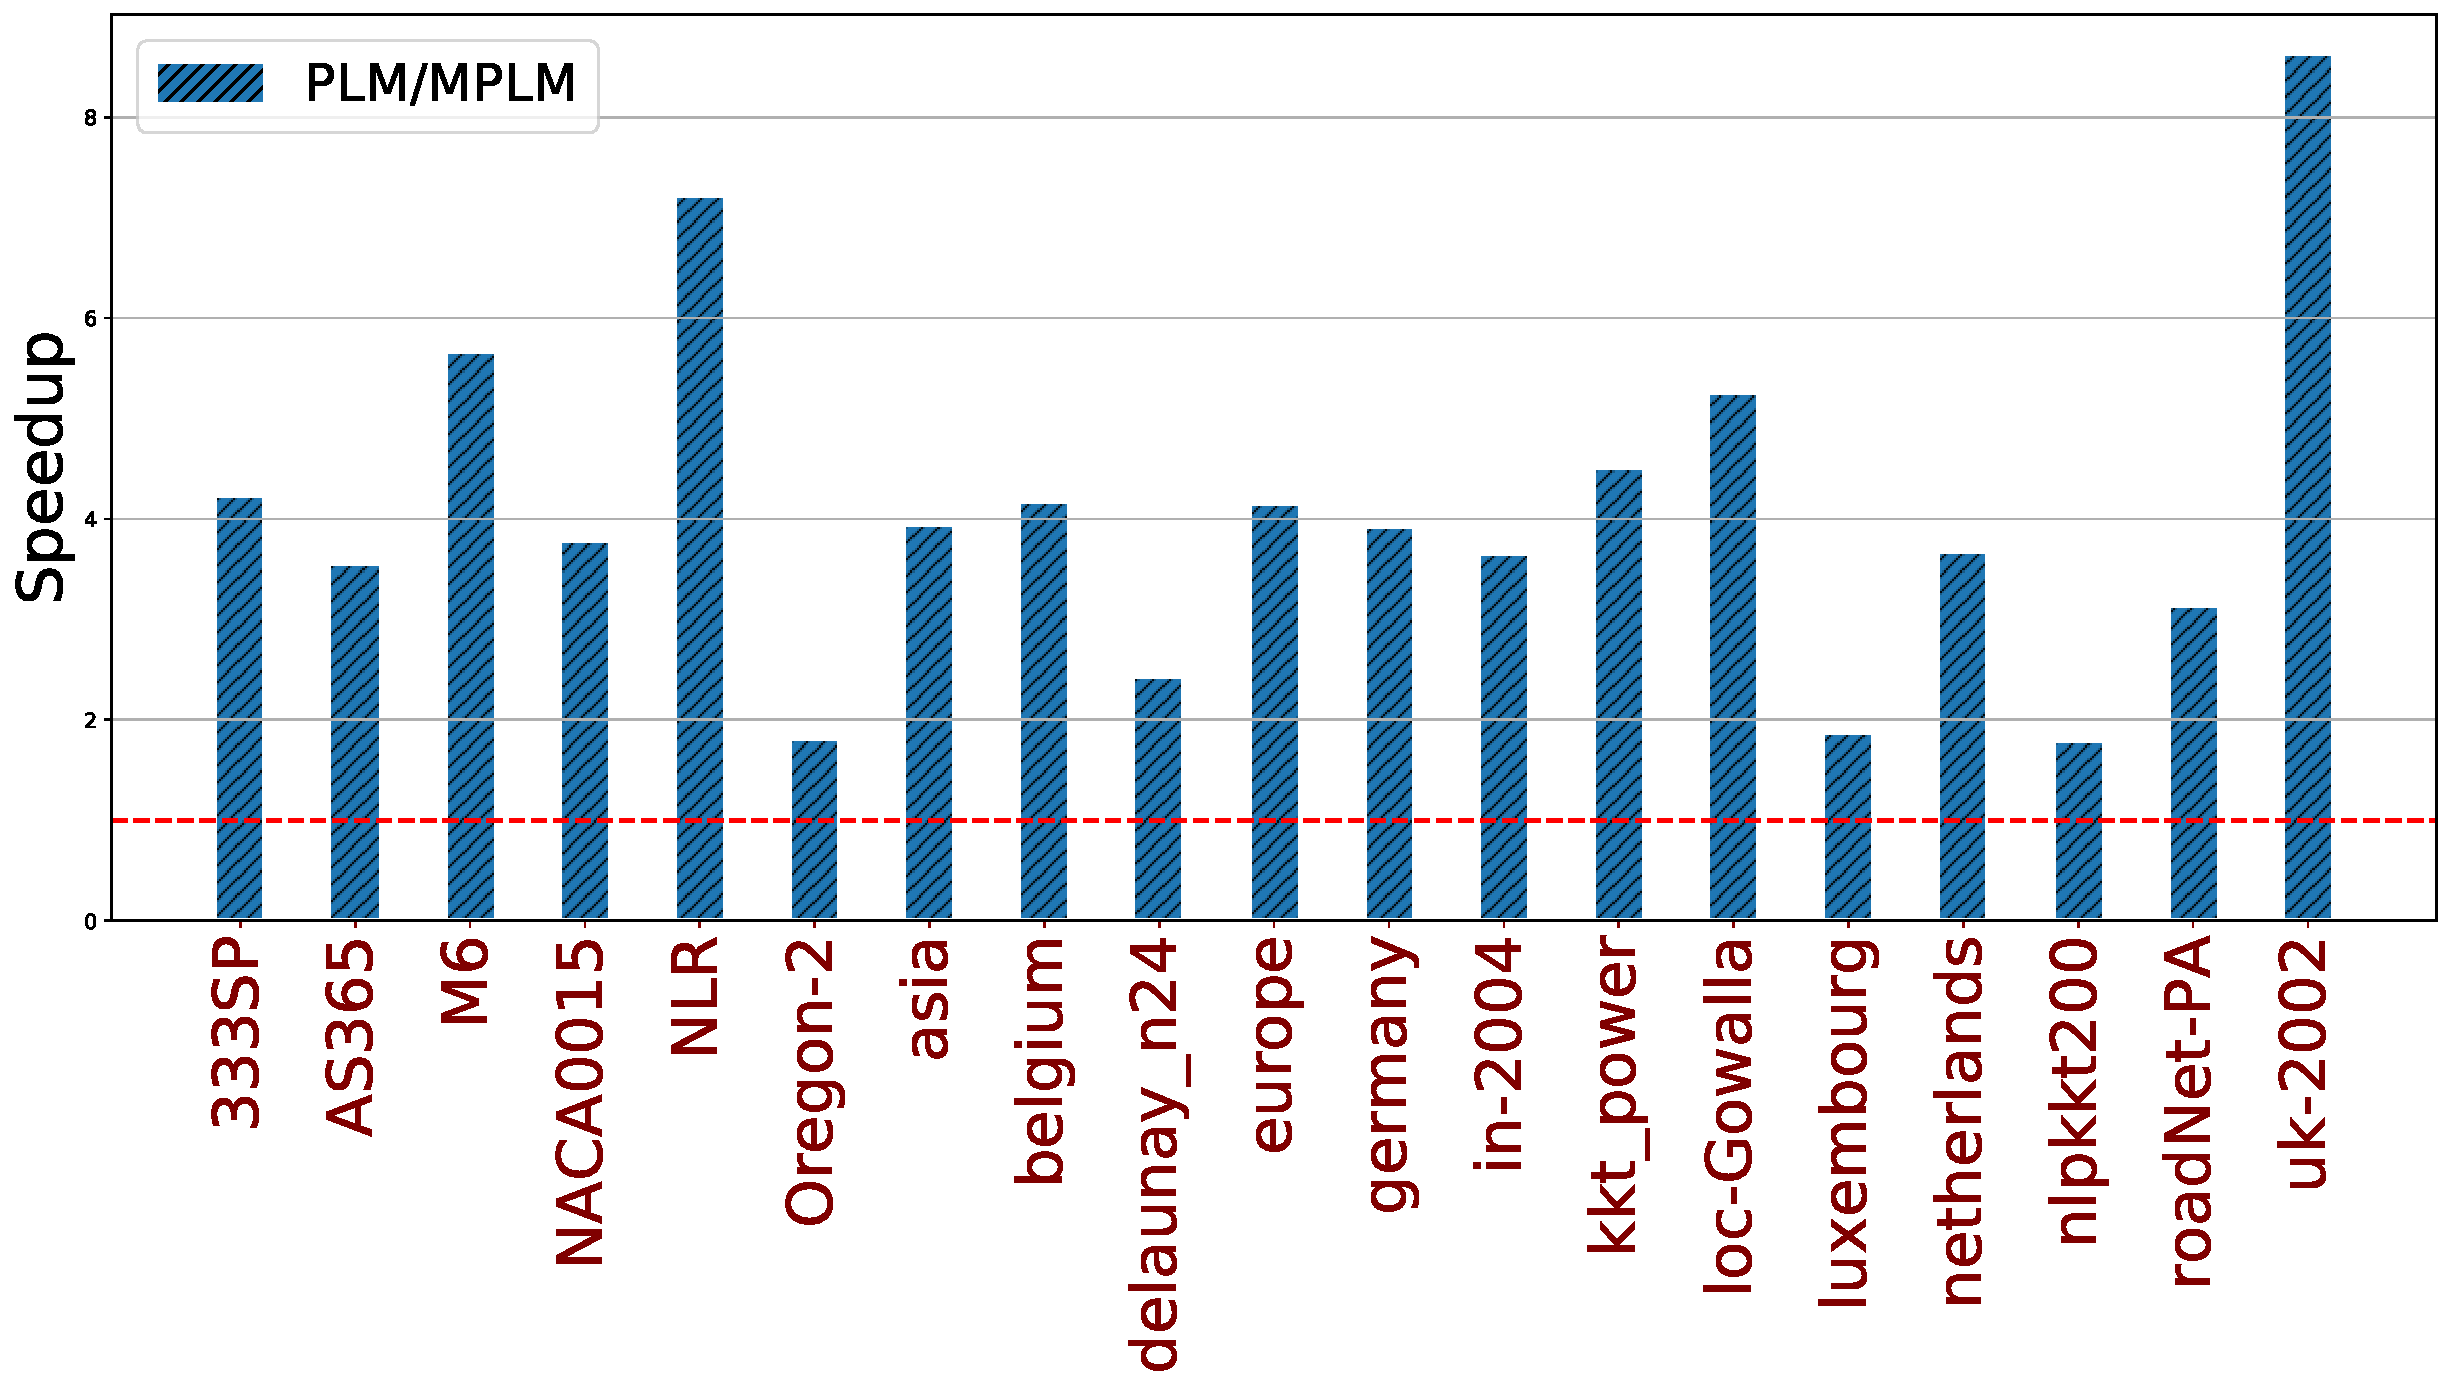
\includegraphics[width=.48\textwidth]{figures/louvain/cascadelake_plm_vs_mplm_threads_48.pdf} \label{fig:plm_vs_mplm_cascade_48_threads_speedup}}
	\subfigure[Modularity of MPLM, ONPL, and OVPL on Cascade Lake(48 threads).]{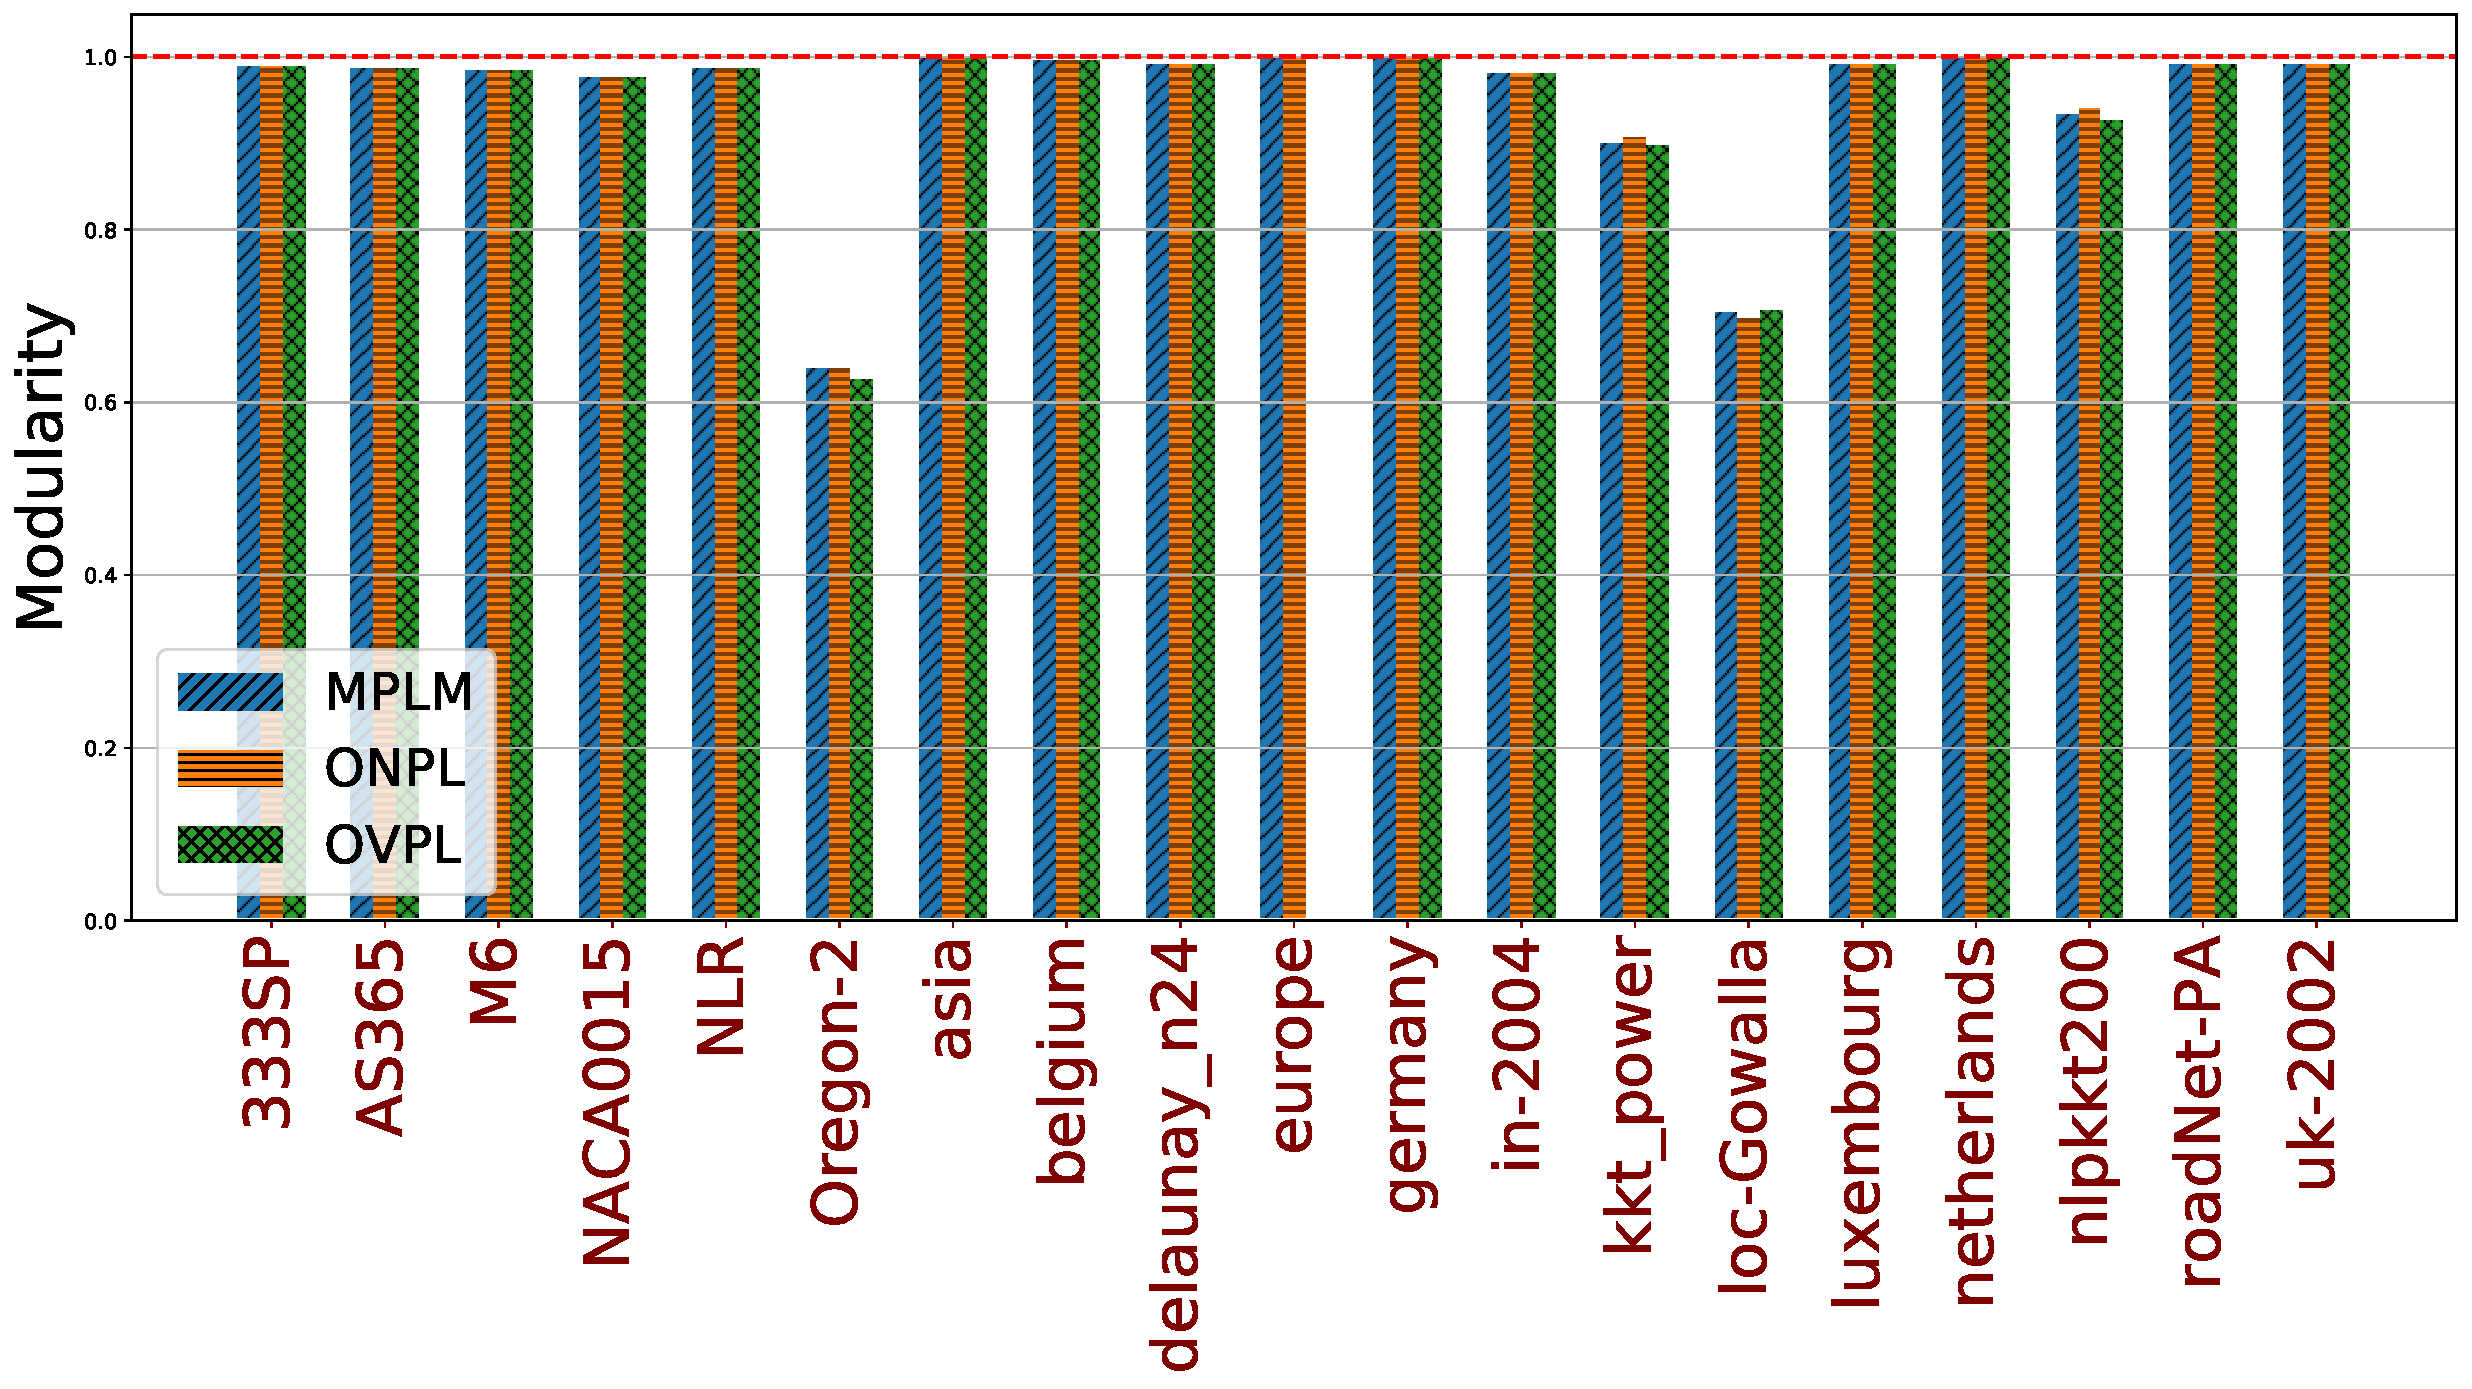
\includegraphics[width=.48\textwidth]{figures/louvain/cascadelake_modularity_mplm_vs_onpl_vs_ovpl_threads_48.pdf} \label{fig:mplm_onpl_vs_ovpl_modularity_cascade_48}}
	\caption{[Louvain Method] Performance and quality of the Modified PLM (MPLM) over PLM.}
  \label{fig:sanity_check_on_cascade_lake_48}
  
\end{figure*}

Figure~\ref{fig:plm_vs_mplm_cascade_48_threads_speedup} presents the improvement of MPLM compared to PLM for 48 threads 
on \textit{Cascade Lake} for all studied graphs. Similar results observe on SkylakeX (not shown for brevity). We will use MPLM as 
the comparison point to see the impact of vector processing in community detection codes. 

\subsubsection{Modularity}
Since the algorithm has significant race conditions, any change of
timings could affect the quality of the communities detected.
Modularity is one of the standard metrics to evaluate the quality of
the communities and is the metric optimized by MPLM.
Figure~\ref{fig:mplm_onpl_vs_ovpl_modularity_cascade_48} shows the
modularity of the implementations of MPLM, ONPL, and OVPL on the
\textit{Cascade Lake} architecture using 48 threads. All methods
achieve almost the same modularity which confirms the quality of the
vectorized communities has not been significantly impacted.

\subsubsection{ONPL}
is a vectorized algorithm with  the same memory consumption as the
scalar algorithm MPLM and similar memory access
patterns. Figure~\ref{fig:mplm_onpl_and_ovpl_cascade_48} shows the
performance of ONPL compared to MPLM on the Cascade Lake for 48
threads: ONPL shows performance improvement for most
of the selected graphs and at most a factor of $2.5$
performance gain compared to \textit{MPLM}.
Figure~\ref{fig:mplm_onpl_and_ovpl_skylake_36} shows the \textit{ONPL}
performance in the NetworKit on the \textit{SkylakeX} architecture.
ONPL performs better than its scalar counterpart for almost all the
graphs.  The best performance of \textit{ONPL} is recorded on the
\textit{SkylakeX} processor is around a factor of $1.8$ compared to
\textit{MPLM}.

\begin{figure}[t]
      \centering
      \subfigure[On Cascade Lake Processor(48 threads).]{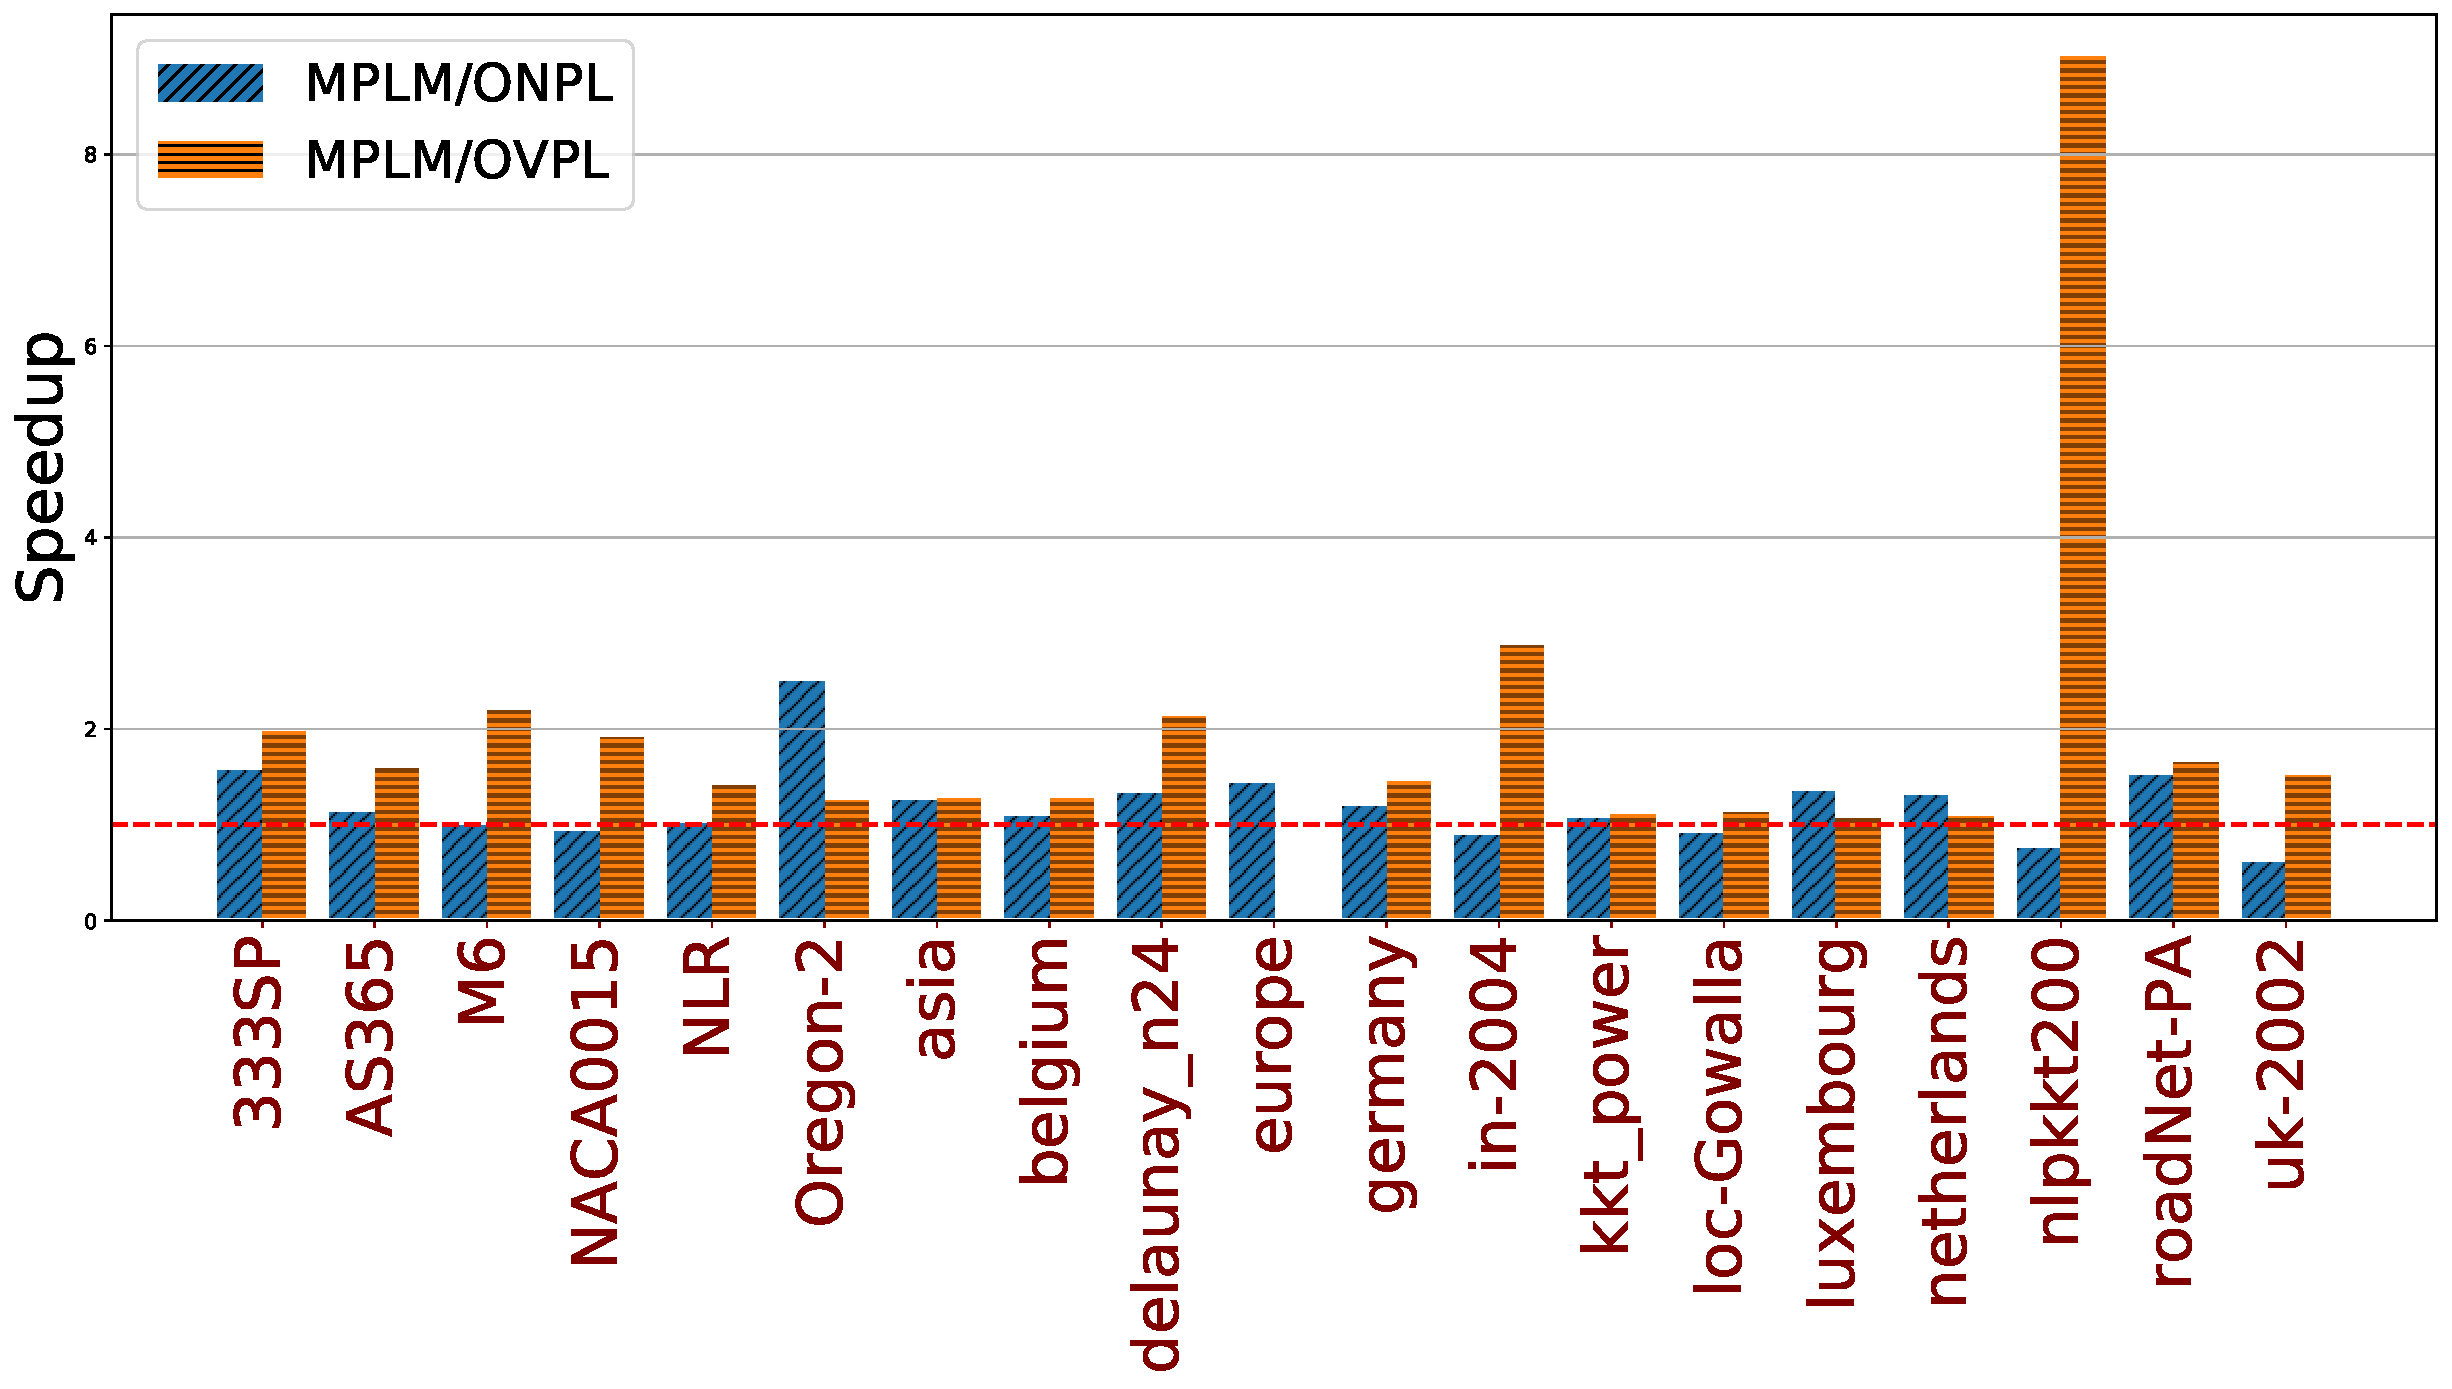
\includegraphics[width=.48\linewidth]{figures/louvain/cascadelake_mplm_vs_onpl_ovpl_threads_48.pdf}\label{fig:mplm_onpl_and_ovpl_cascade_48}}
      \subfigure[On SkyLakeX Processor(36 threads).]{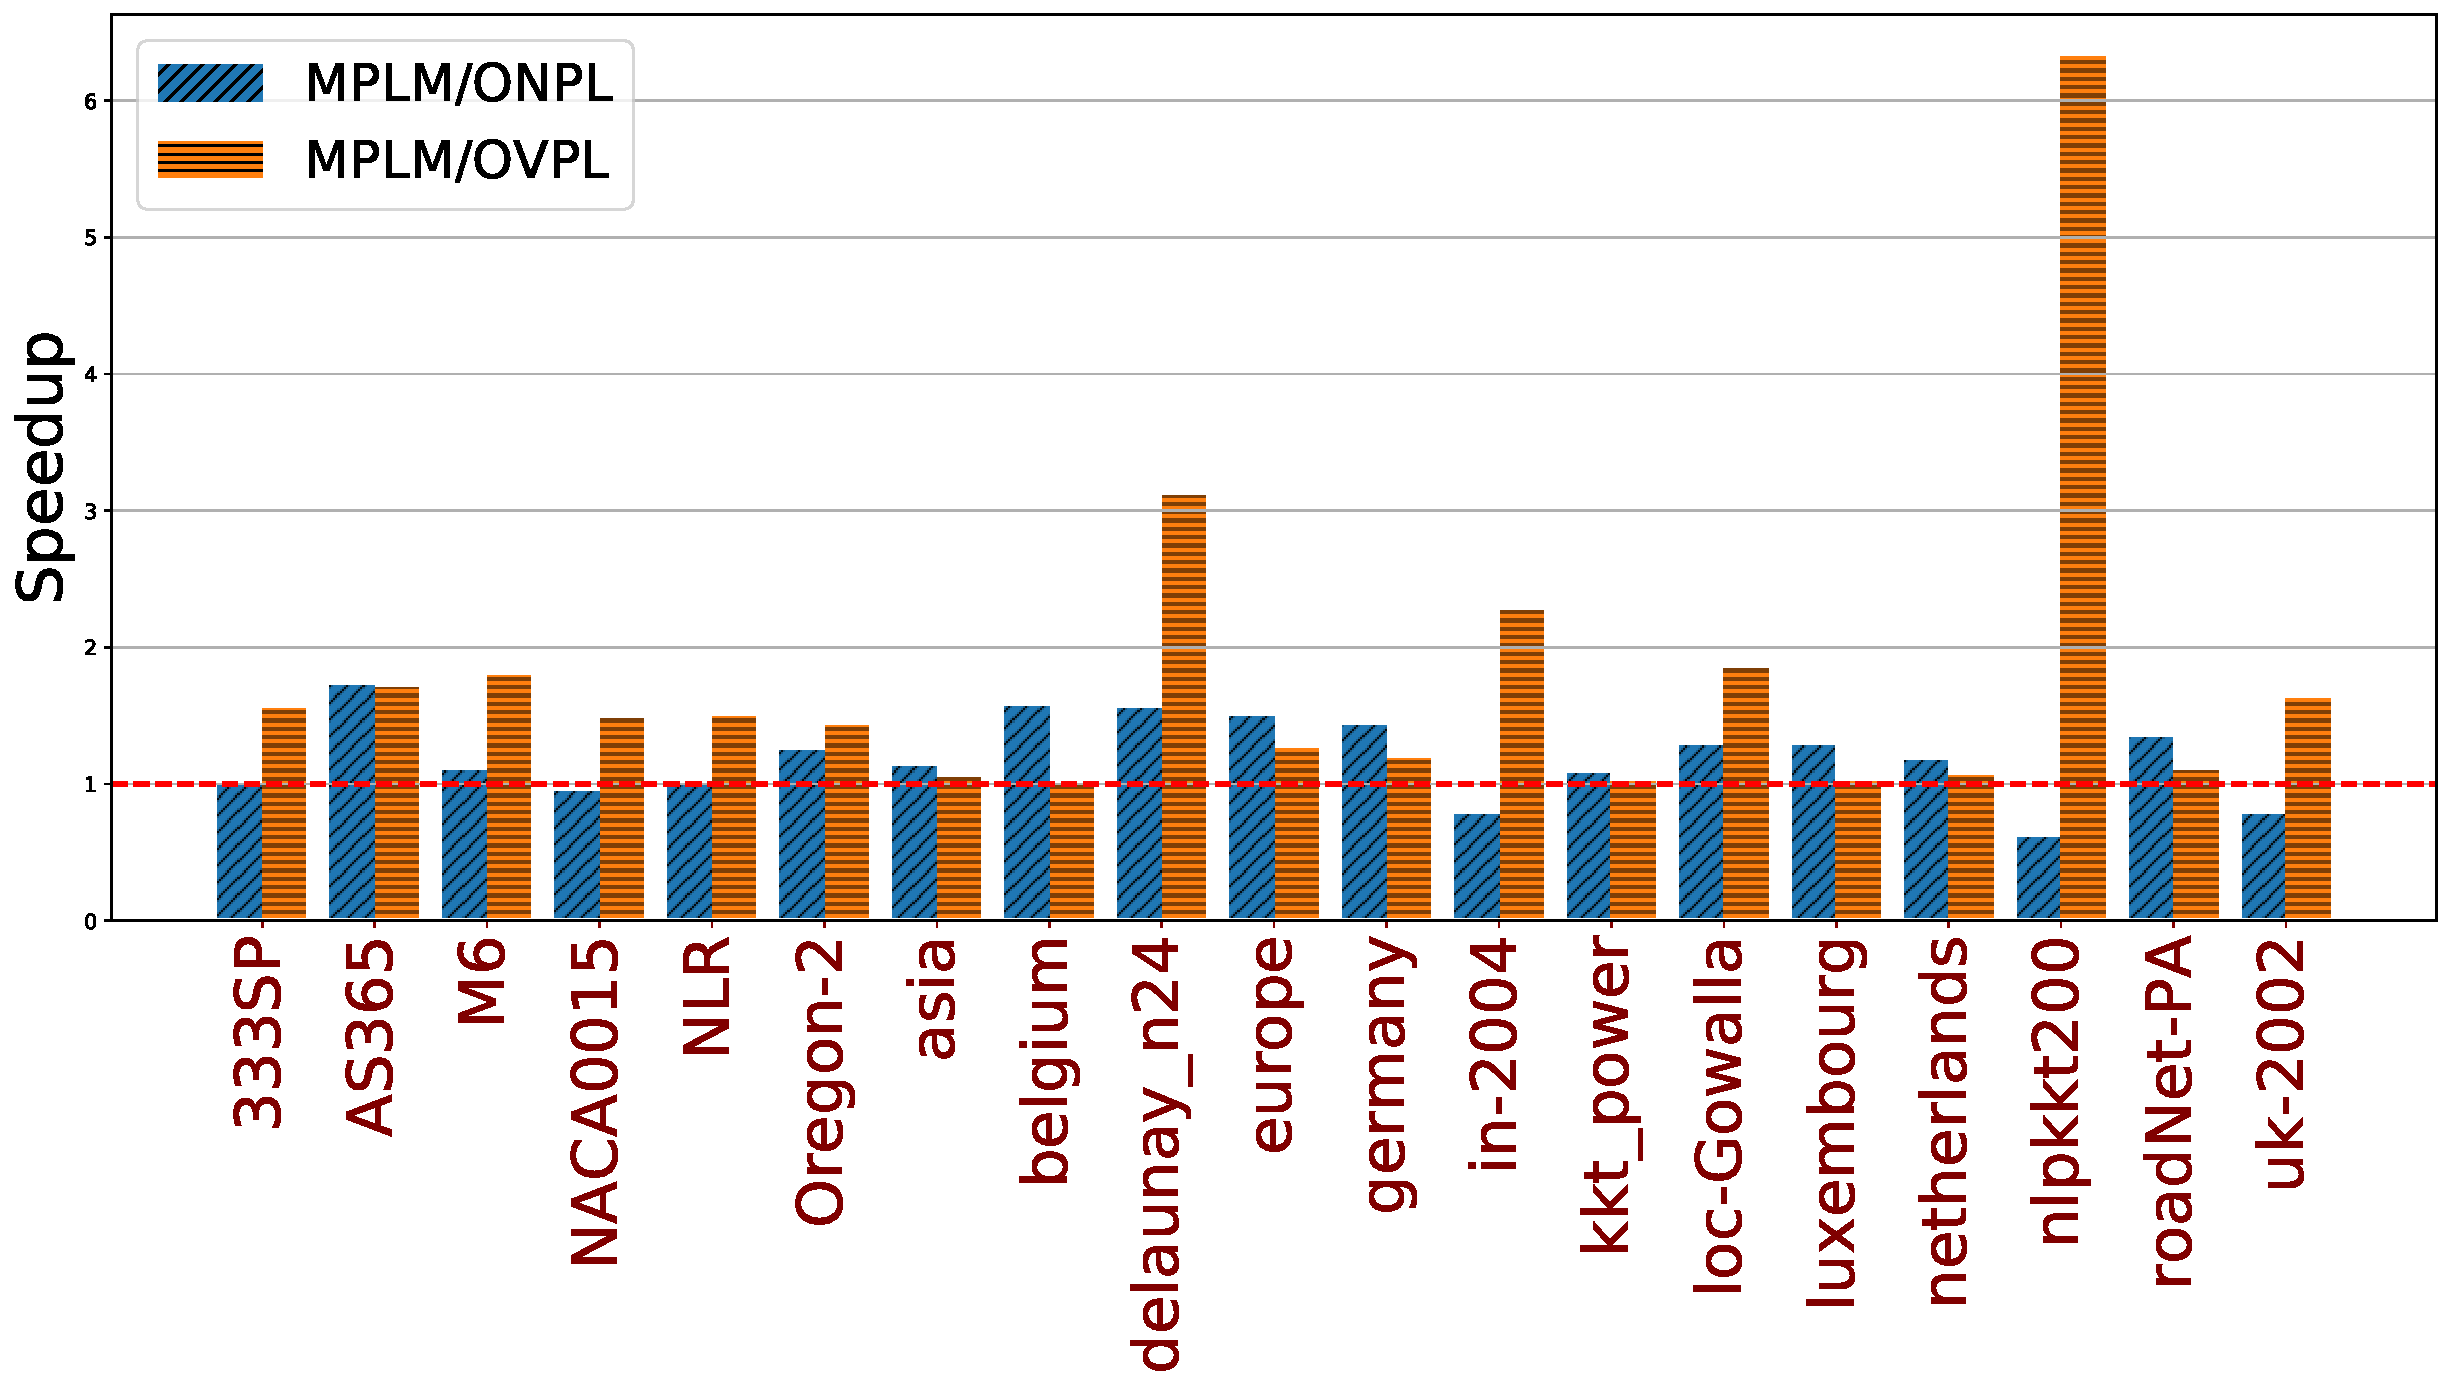
\includegraphics[width=.48\linewidth]{figures/louvain/skylake_mplm_vs_onpl_ovpl_threads_36.pdf} \label{fig:mplm_onpl_and_ovpl_skylake_36}} 
      \caption{[Louvain Method] Speedup of ONPL and OVPL over MPLM.}   
      \label{fig:speedup_mplm_onpl_ovpl}
 \end{figure}

\subsubsection{OVPL}
is an algorithm that consumes a lot more memory than the scalar
algorithm due to having to store community affinity information for an
entire block of
vertices. Figure~\ref{fig:mplm_onpl_and_ovpl_cascade_48} presents the
results of OVPL on the \textit{Cascade Lake} architecture relative to
the scalar implementation. For the graphs that were completed (some graphs
ran out of memory), the performance derived is much better than the
scalar implementation. Figure~\ref{fig:mplm_onpl_and_ovpl_skylake_36}
shows the performance of OVPL on SkylakeX. We can
see a factor of $9.0$ and $6.5$ performance gain for \textit{OVPL} on
the \textit{Cascade Lake} and \textit{SkylakeX} processors
respectively compared to \textit{MPLM}.

\begin{figure}[t]
  \centering
  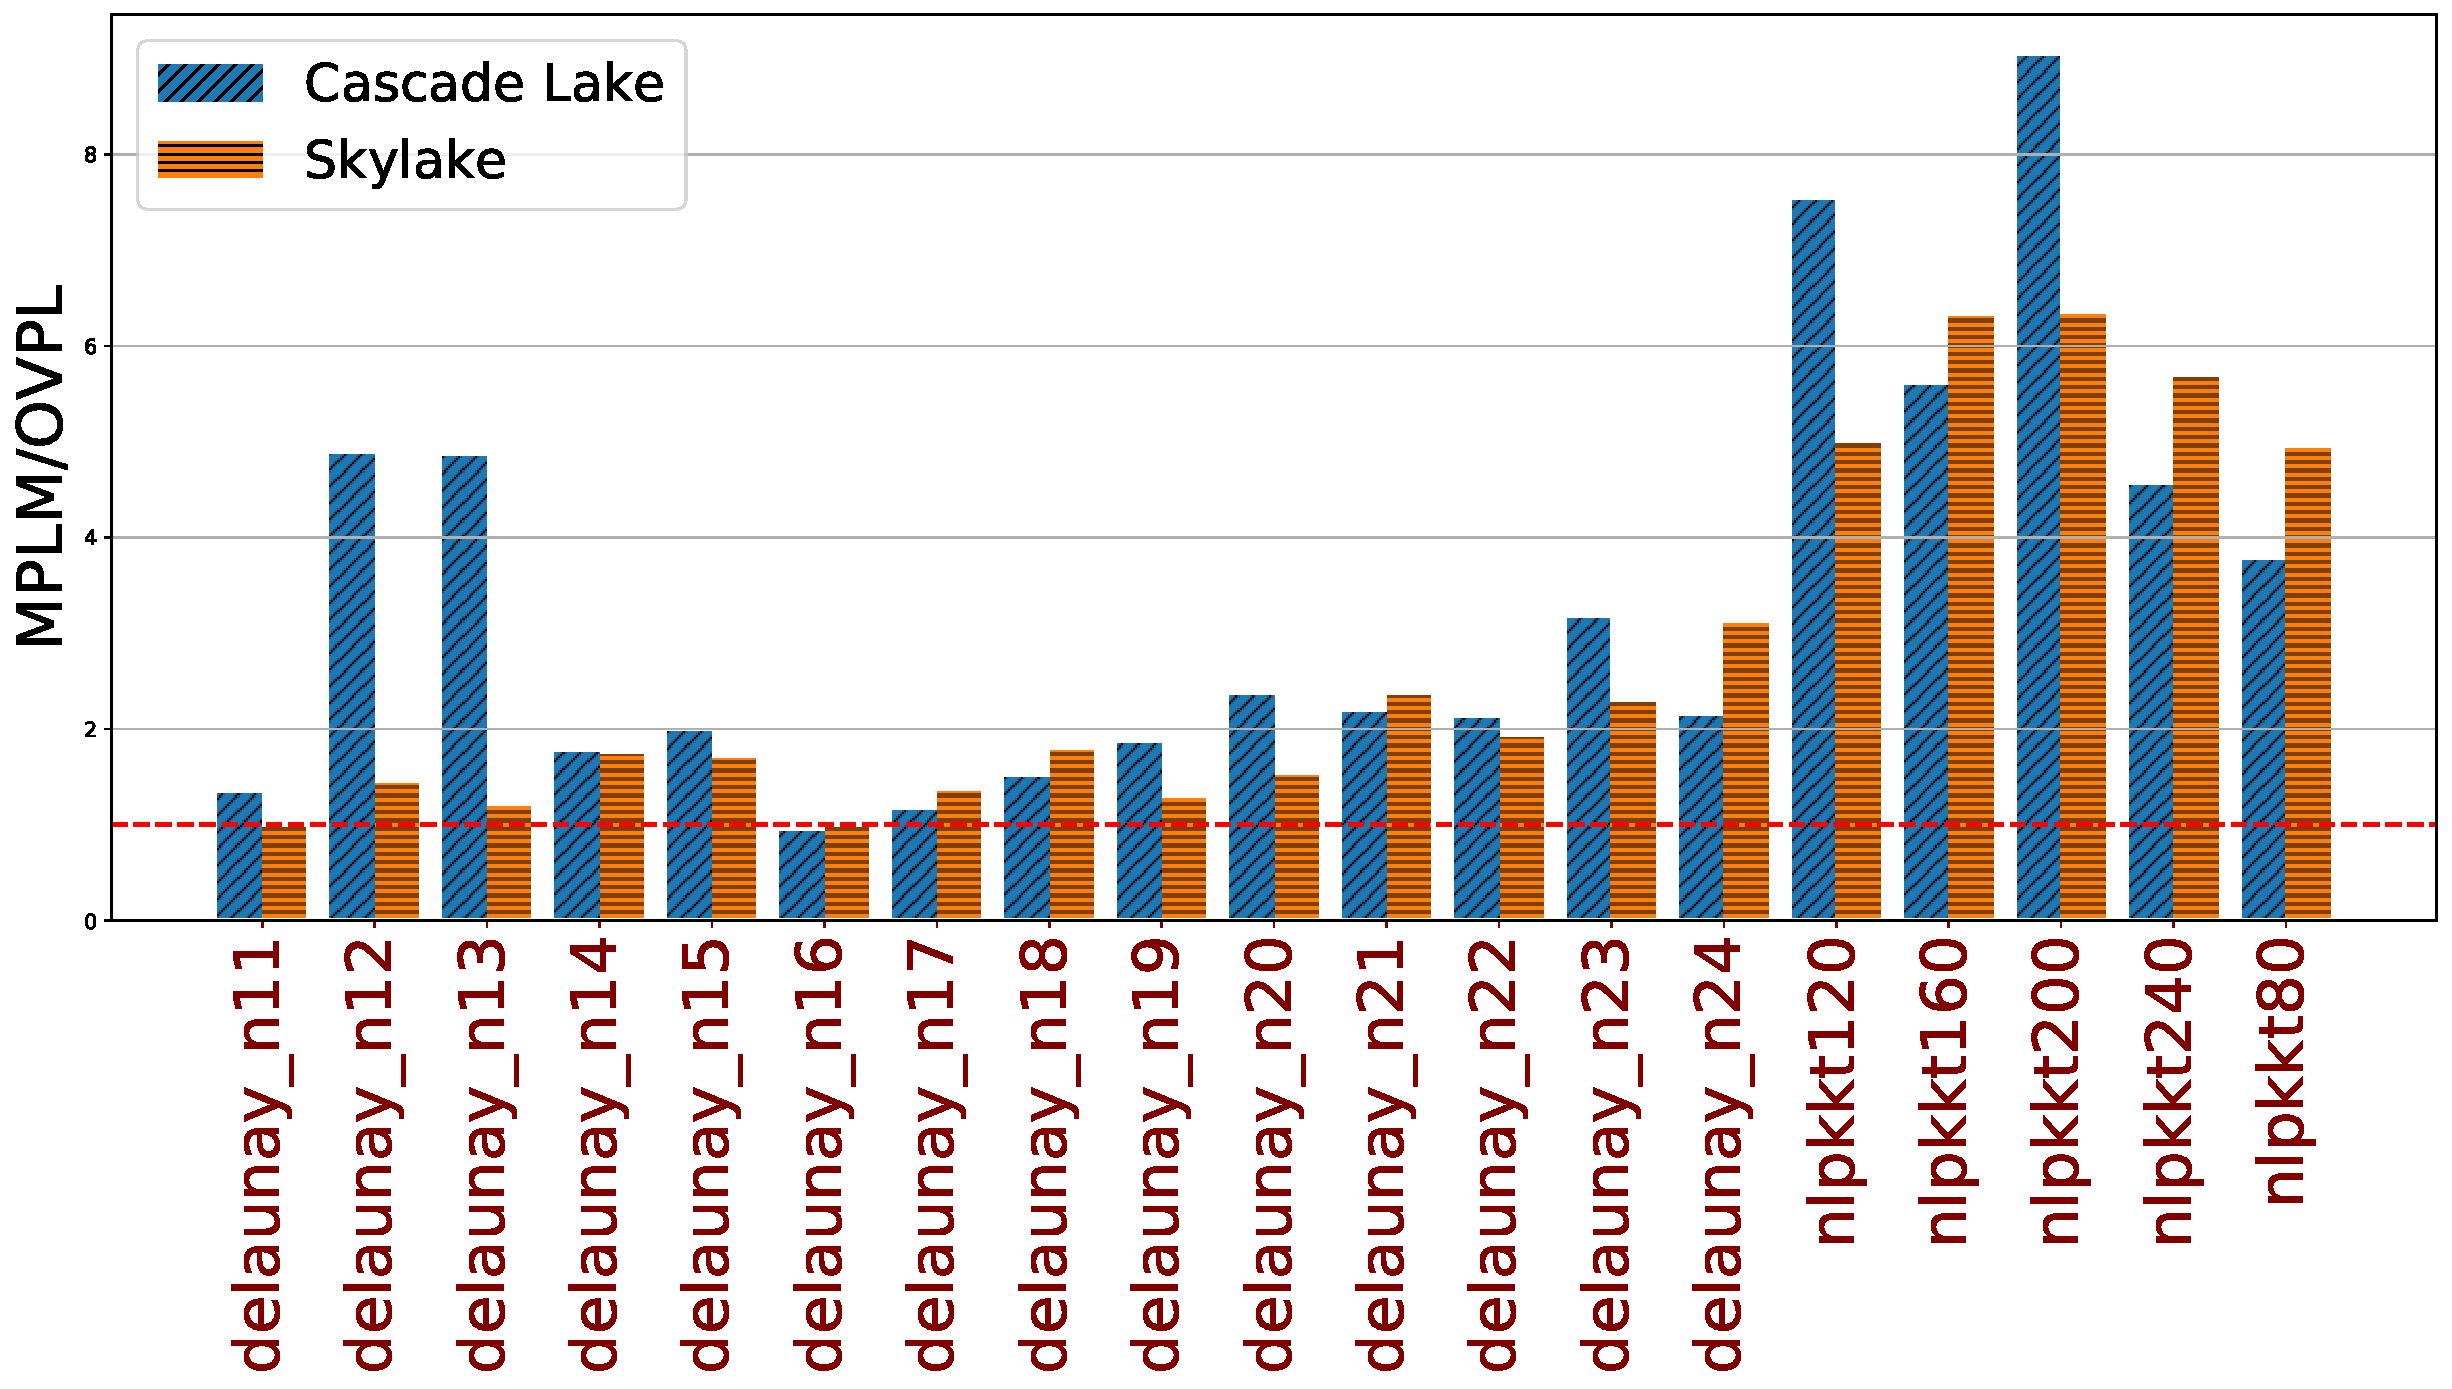
\includegraphics[width=.48\linewidth]{figures/louvain/selected_mplm_vs_ovpl_cascade_48_skl_36.pdf}
  \caption{[Louvain Method] Speedup of \textit{OVPL} over \textit{MPLM} for the selected graphs where many vertices have degrees close to the average on both architectures.}
  \label{fig:mplm_vs_ovpl_cascade_48_skylake_36}
\end{figure}

From the algorithm perspective, \textit{OVPL} performs vectorization on a block of vertices, more specifically proper vectorization 
applies on the iteration only the minimum degree of vertices from the block. The rest of the iterations need more branching 
and also some lanes of the vectorization always remain unused. Our experimental results also reflect the scenario. Figure~\ref{fig:mplm_vs_ovpl_cascade_48_skylake_36} 
shows only the performance of the selected graphs where most of the vertices have the same degree or very small variations. 
It shows a great performance gain. Graphs like \texttt{Delaunay}(average Degree 5) triangulations of random points or sparse matrix 
\texttt{nlpkkt}(average Degree 26) have most vertices with degrees close to the average. Every vertex in \textit{OVPL}’s block is in sorted 
order and properly distributed by their degree, which also brings great load balancing. 

\subsubsection{Energy Consumption}
\begin{figure}[t]
      \centering
      \subfigure[MPLM vs ONPL.]{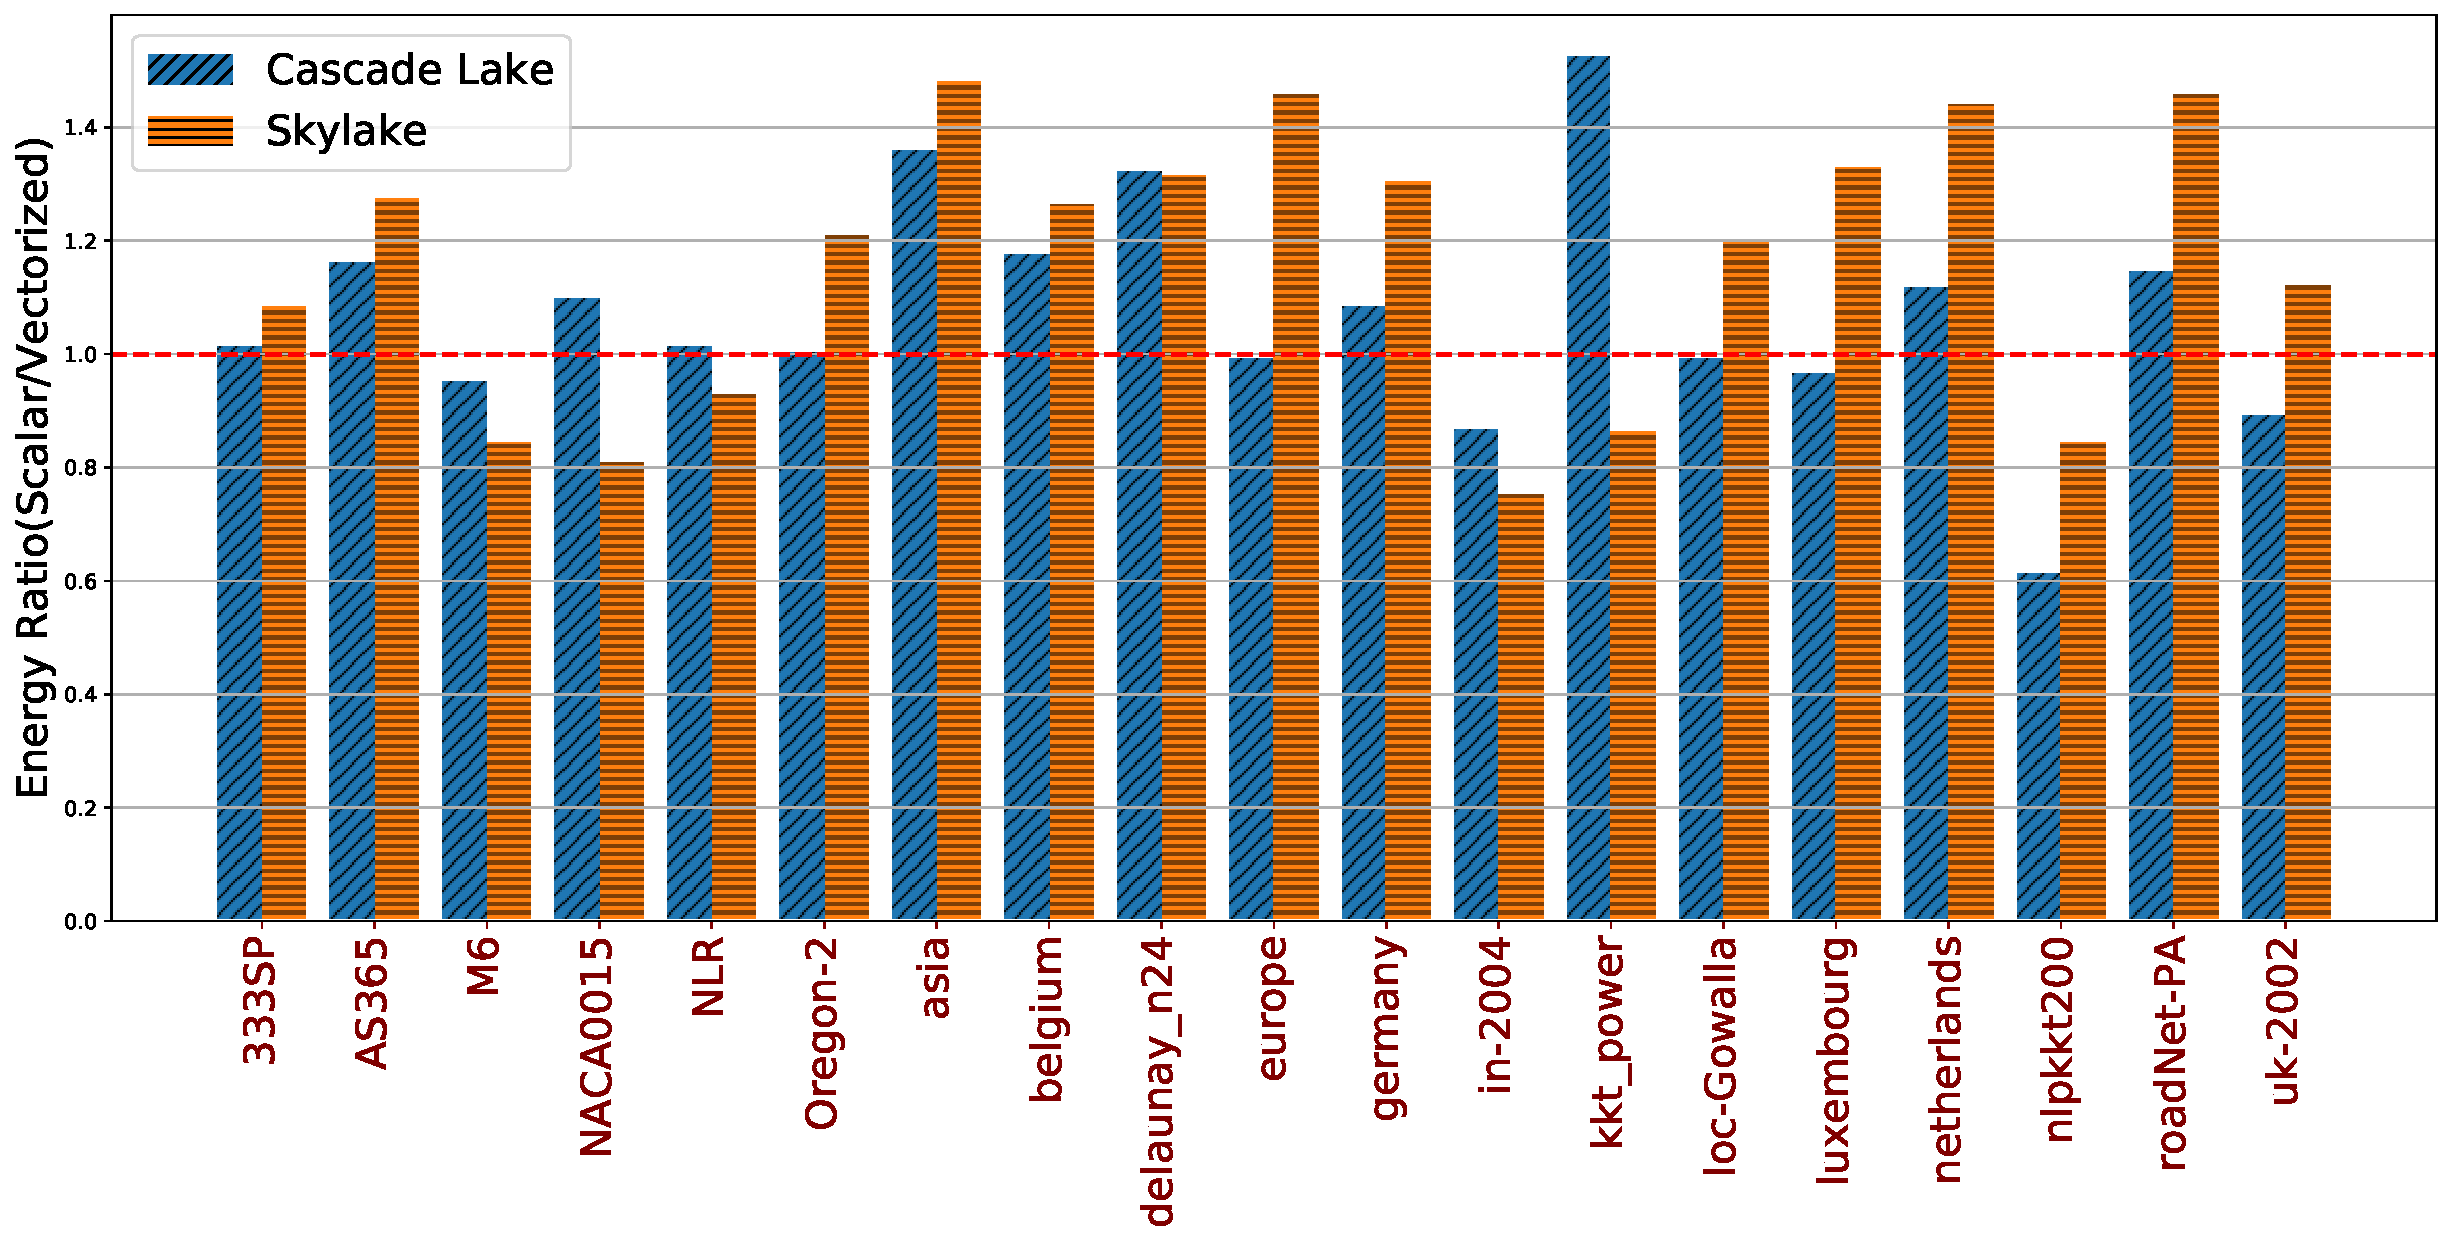
\includegraphics[width=.48\linewidth]{figures/louvain/power/mplm_vs_onpl_power_cascade_48_skl_36_mean.pdf}\label{fig:power_mplm_vs_onpl}}
      \subfigure[MPLM vs OVPL.]{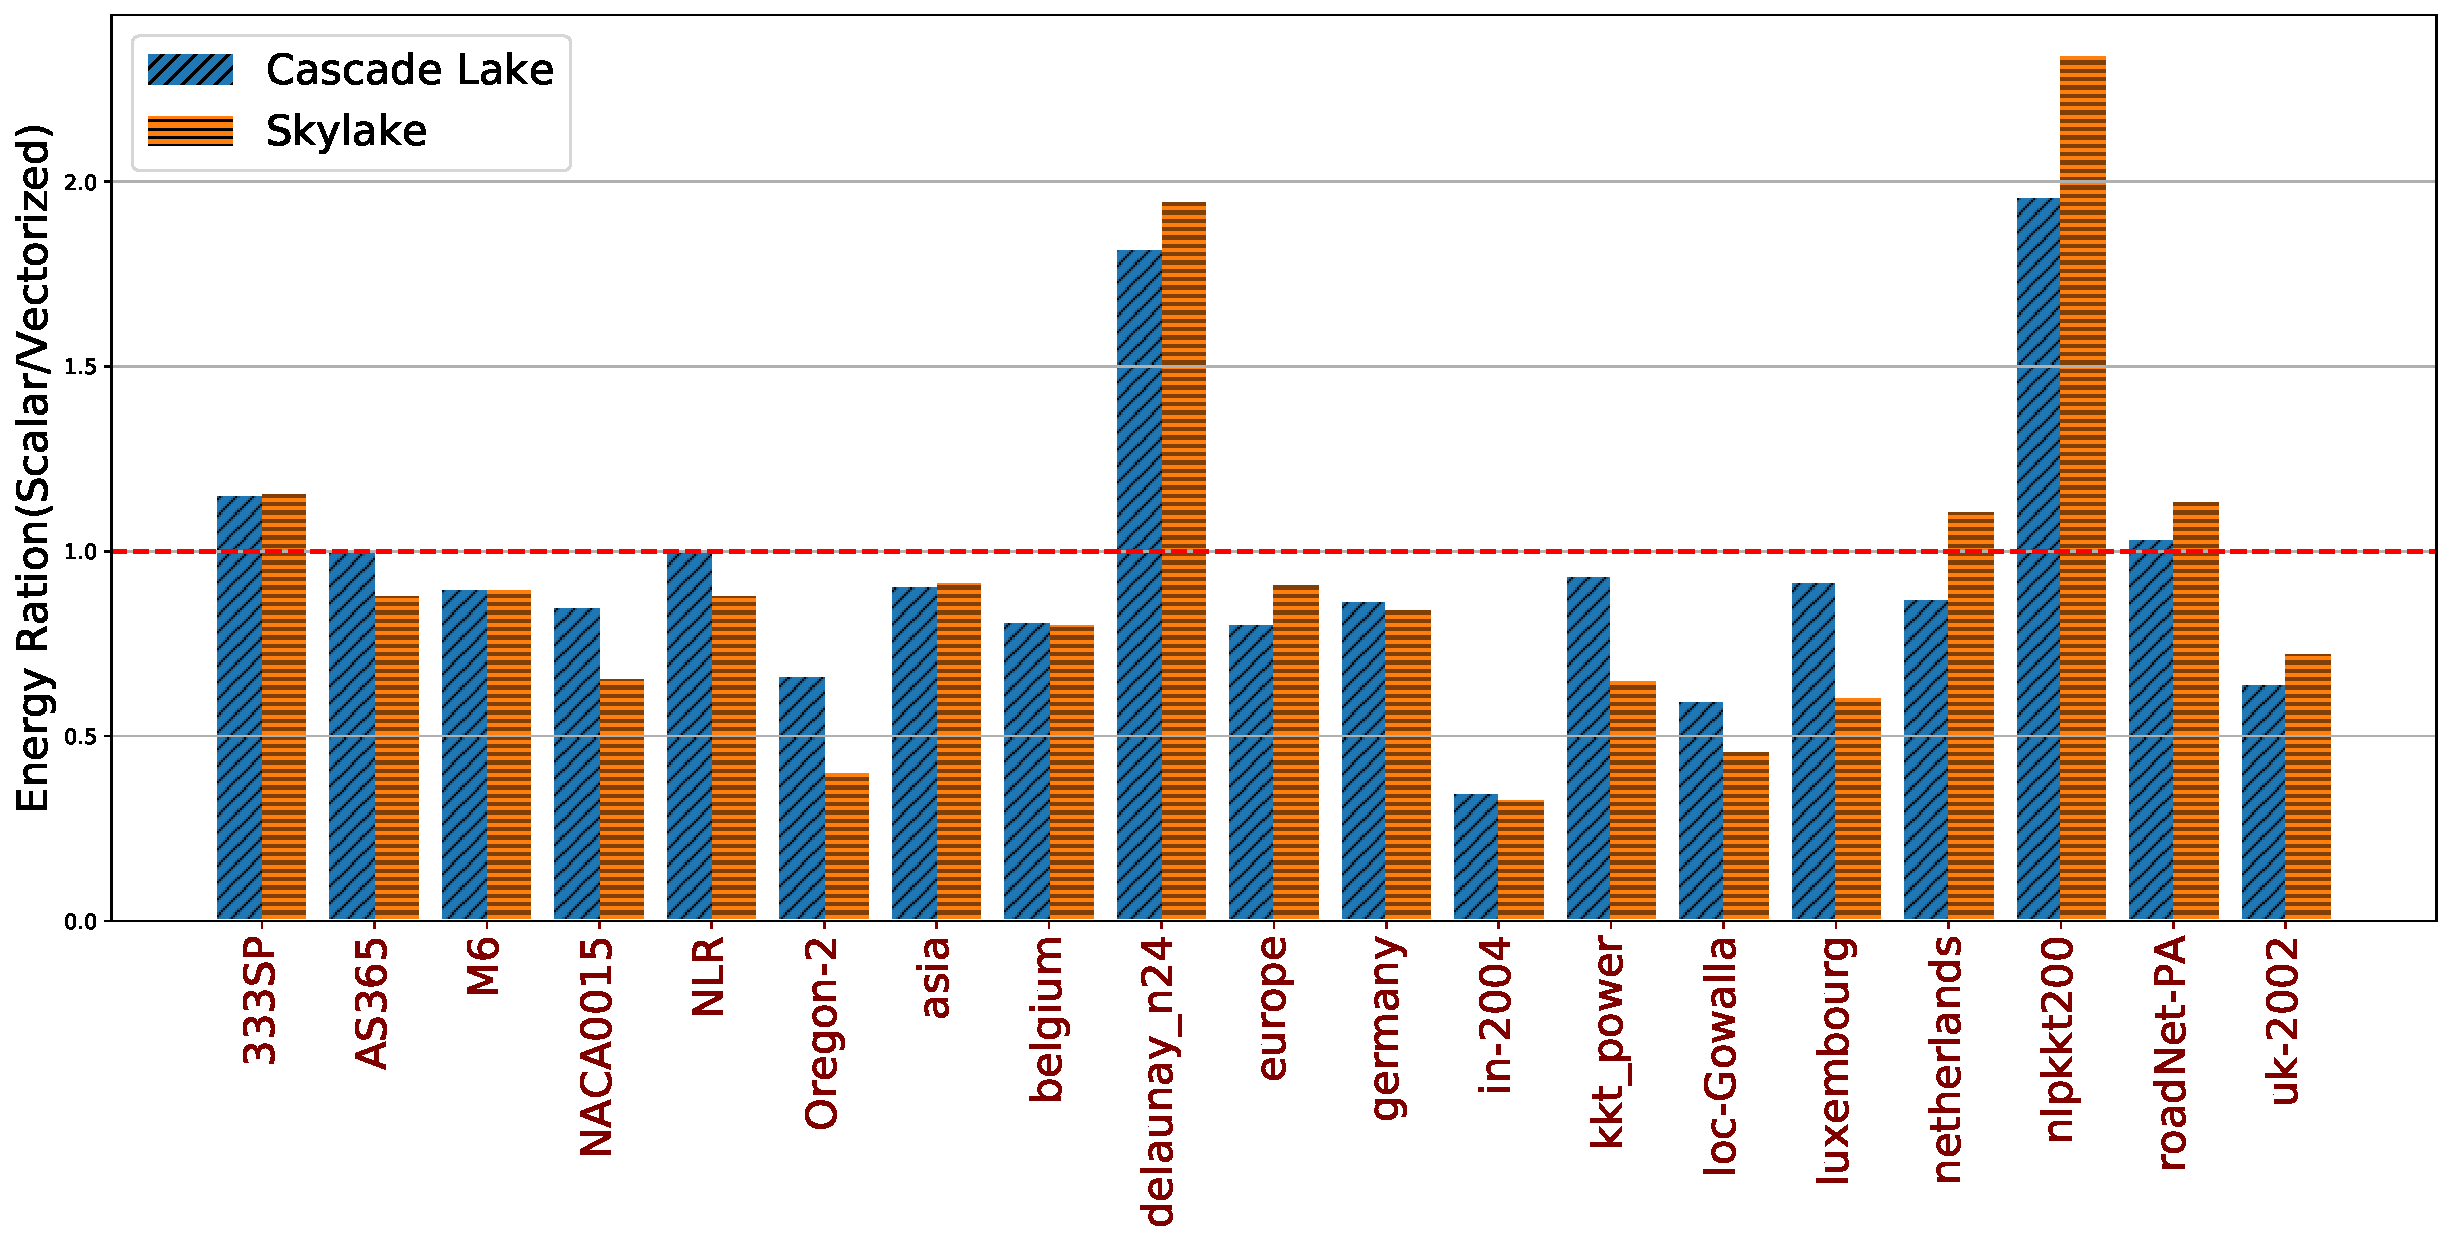
\includegraphics[width=.48\linewidth]{figures/louvain/power/mplm_vs_ovpl_power_cascade_48_skl_36_mean.pdf} \label{fig:power_mplm_vs_ovpl}} 
      \caption{[Louvain Method] Energy consumption comparison of ONPL and OVPL over MPLM on Skylake(36 threads) and Cascade Lake(48 threads).}   
      \label{fig:power_on_skylake_cascade}
 \end{figure}

Figure~\ref{fig:power_on_skylake_cascade} shows the overall energy
consumption of different Louvain methods.  The energy consumption by
Louvain methods is calculated from RAPL (Running Average Power Limit)
energy usages.  Figures~\ref{fig:power_mplm_vs_onpl}
and~\ref{fig:power_mplm_vs_ovpl} show the energy consumption of ONPL
and OVPL over MPLM. Any bar above 1 represents ONPL or OVPL consuming
less energy than MPLM. Using SIMD operations helps to reduce the
number of instructions in the execution. So, the expectation is that it
can give better run time as well as better energy usage.

OVPL consumes more energy compared to ONPL and MPLM. Indeed, OVPL
needs extra pre-processing, so it is adds work to enable
vectorization. Also, because the vectorization pads the graph
representation to fit the vector lanes, there are cases where vector
lanes are actively used to perform no useful computation, which raises
energy consumption. Since OVPL adds work and wastes vector lane, it
makes sense that it raises energy consumption.


ONPL shows decent energy efficiency for both architectures (Cascade
Lake and Skylake). Most graph tested have a better energy consumption
with ONPL than with MPLM. If we compare
Figures~\ref{fig:speedup_mplm_onpl_ovpl}
and~\ref{fig:power_on_skylake_cascade}, we can see that some graphs
see better energy gains than speedup. For instance, \textit{uk-2002}
see a slowdown from ONPL but a factor of 1.2 of gain in energy
efficiency. That means vectorization can help graph algorithms by not
only making them faster but also energy efficient. We conjecture that
while vector instruction consume more power, they decrease the number
of instruction that need to be decoded which can translate in energy gains.


\subsection{Label Propagation on NetworKit}
\begin{figure}[t]
  \centering
	\subfigure[On Cascade Lake Processor(48 threads).]{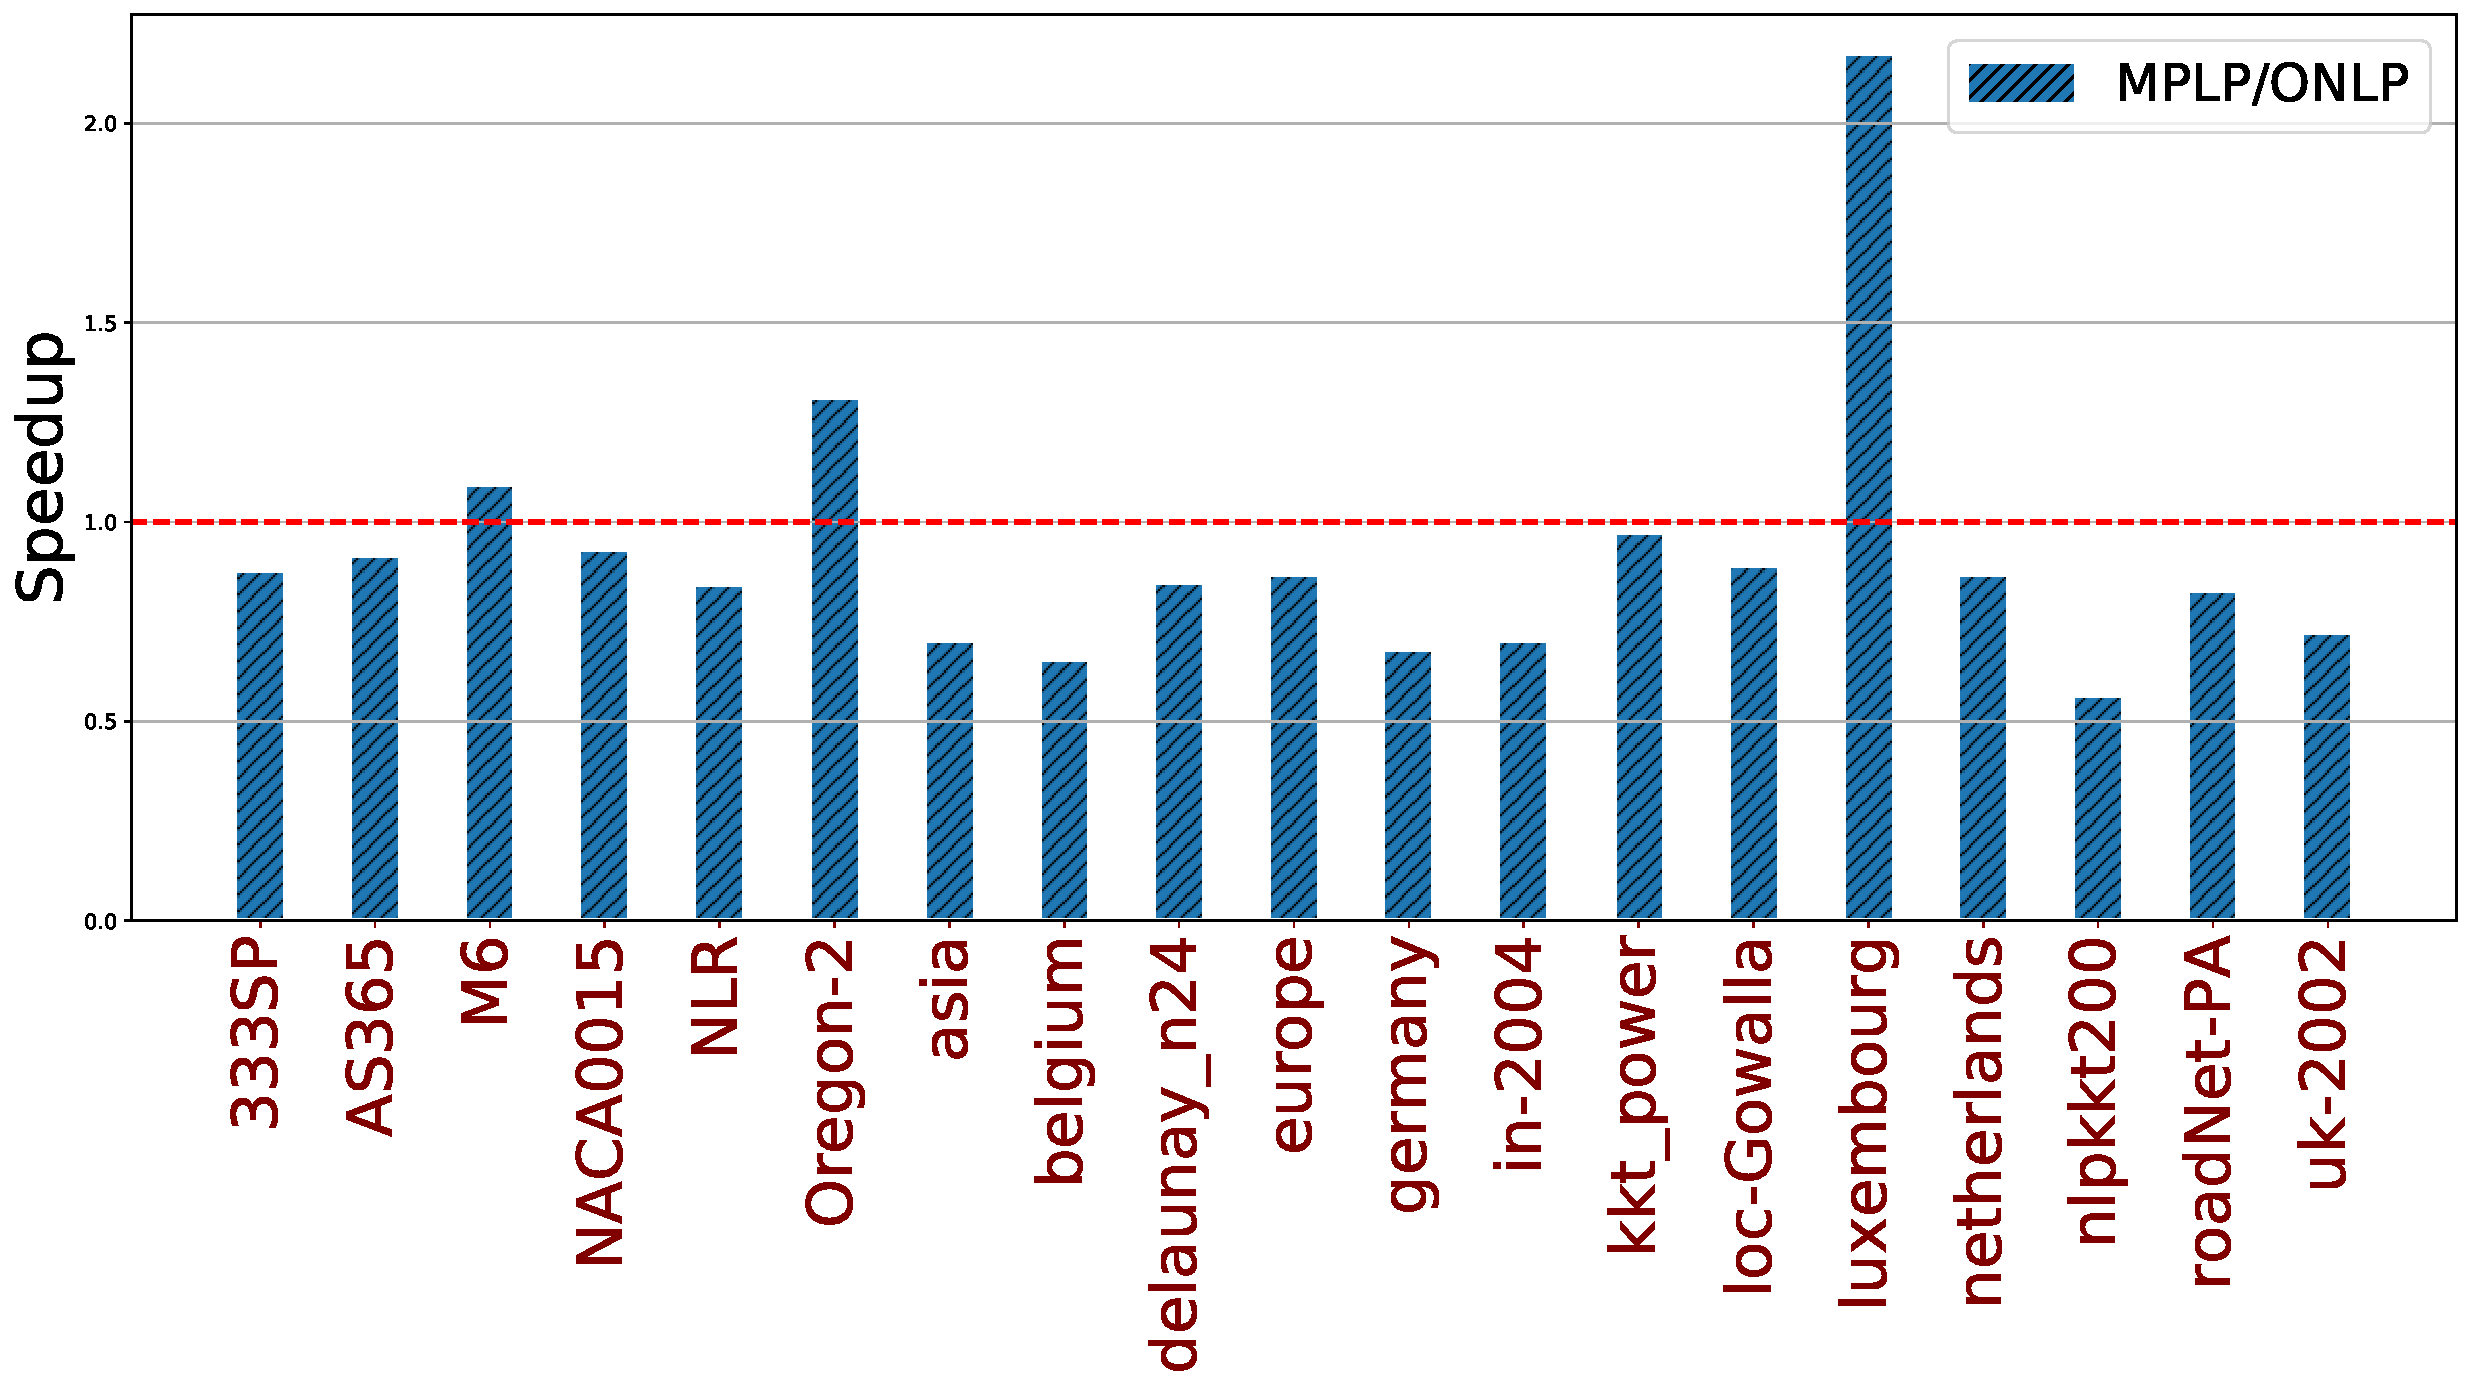
\includegraphics[width=.48\linewidth]{figures/LP/cascadelake_mplp_vs_onlp_threads_48_iter_1.pdf}\label{fig:lp_cascade_mplp_vs_onlp}}	 
  	\subfigure[On SkyLakeX Processor(36 threads).]{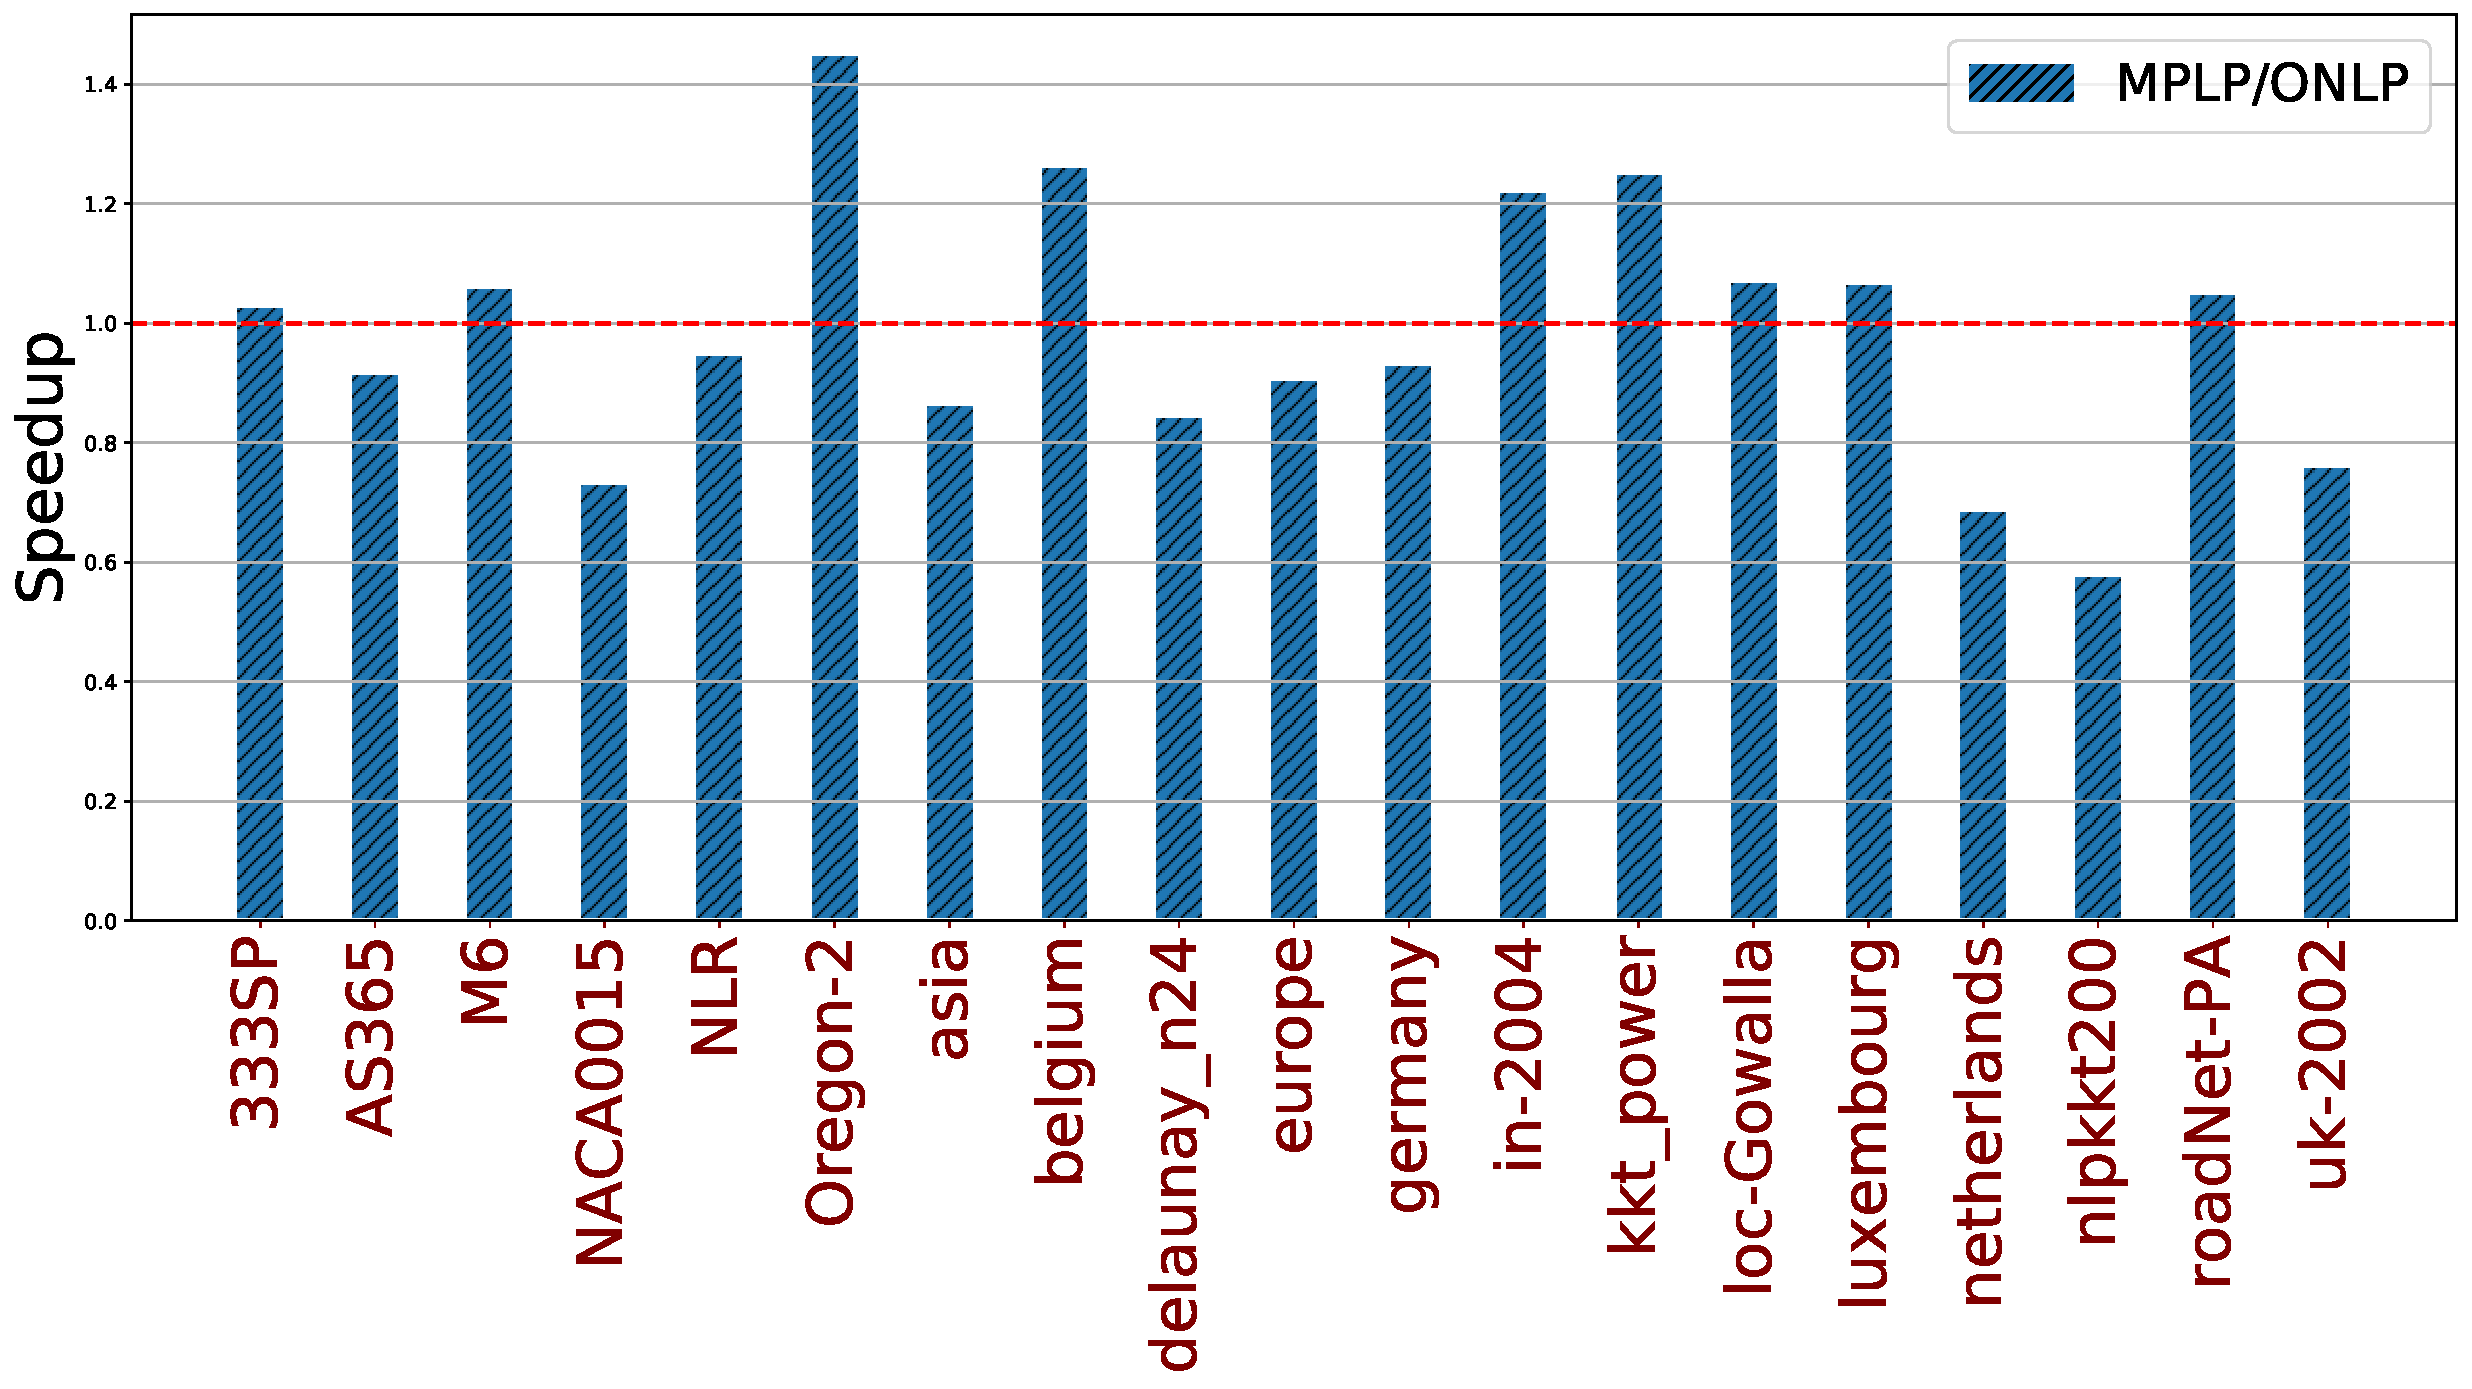
\includegraphics[width=.48\linewidth]{figures/LP/skylake_mplp_vs_onlp_threads_36_iter_1.pdf} \label{fig:lp_skylake_mplp_vs_onlp}} 
    \caption{[Label Propagation] Speedup of vectorized Label Propagation(ONLP) over the parallel Label Propagation(MPLP).} 
  	\label{fig:lp_mplp_onlp_skl_cascade}
\end{figure}

Figure~\ref{fig:lp_mplp_onlp_skl_cascade} shows the performance of
label propagation(LP) on Cascade Lake and SkylakeX processors. The
parallel and vectorized one neighbor per-lane label propagations
represent by MPLP and ONLP. A couple of graphs get moderate
performance gain for ONLP on Cascade
Lake~\ref{fig:lp_cascade_mplp_vs_onlp} processor; the highest
performance gain is reported around 2.0 times over MPLP. Graphs on
SkylakeX processor~\ref{fig:lp_skylake_mplp_vs_onlp} also show
moderate performance.

It is possible to vectorize the Label Propagation, but it has limited
benefits. In the Louvain method, we vectorize the affinity calculation
and modularity calculation code sections. Both of the code sections
are required a good amount of instructions to assign vertices to their
respective community. So while gather and scatter provide limited
performance benefits, they enable the rest of the affinity and
modularity calculation to be vectorized which improves
performance. However, the vectorization of the Label Propagation does
not lead to many more instructions to be vectorized. 

\section{Related Work}

Label propagation is one of the most popular community detection
algorithm proposed by Raghavan \textit{et
  al.}~\cite{raghavan2007near}.  The algorithm iteratively refines
labeling of vertices to communities by finding for each vertex the
label that most frequently appears in its neighborhood and migrating
the vertex to that label. PLM~\cite{plm} is the shared-memory
parallelization of the Louvain Method~\cite{Vincent} we use as a reference. Halappanavar \textit{et
  al.}~\cite{halappanavar2017scalable} presented community detection
for static and dynamic networks using Grappolo.

Cheong \textit{et al.}~\cite{cheong2013hierarchical} proposed
a parallel Louvain method for GPUs using three levels of
parallelism for the single and multi-GPU architectures. Later, Naim
and Manne \textit{et al.}~\cite{Naim17} proposed a highly scalable GPU
algorithm for the Louvain method, which parallelizes the access to
individual edges. There are other recent works like 
Sanders \textit{et al.}~\cite{low2020linear} proposed Louvain method for the python; 
the main objective of their work is the simplicity to implement the algorithm in 
python language. Gheibi \textit{et al.}~\cite{gheibi2020cache} proposed a cache efficient 
Louvain method for Intel Knight Landing(KNL) and Haswell architecture.

Both GPUs and CPUs are SIMD systems, at least in spirit. Taking the
analogy of a GPU warp as a core and a thread inside a warp as a lane,
algorithms for GPUs can be re-envisioned as vectorized CPU
algorithm. At a very high level, the distinction between
vertex-based algorithms (such as OVPL) and edge-based algorithms (such
as ONPL) appears in GPUs. However, there are still many differences
between the architectures which cause engineering and algorithmic
decisions for CPU and GPU systems very different.


\section{Conclusion}
We considered the impact of AVX-512 instructions on graph partitioning
problems. We investigated, in particular, the \textit{Cascade Lake}
and the \textit{SkylakeX} architectures and how to use them to perform
speculative greedy graph coloring, the Louvain method, and Label Propagation.

Using different SIMD lanes for different vertices only makes sense for
the Louvain Method as this vectorization requires a pre-processing
overhead. The vectorization forces to process blocks of vertices with
the same number of neighbors, which induces some work overhead. It
proved to be particularly efficient for graphs with balanced degrees
and high average degrees.

The vectorization strategy that processes multiple neighbors of a
single vertex at once also shows performance improvement for many
graphs. That strategy is only possible thanks to scatter instructions
and other various new instructions in \texttt{AVX-512} that are
critical to partitioning problems. The reduce and scatter pattern is
critical in implementing these vectorizations.

Reduce-scatter as a concept can be implemented in multiple ways with
vector instructions. We implemented both in our software environment
by using intrinsic operations. In future works, we want to investigate
compiler techniques to enable us to deploy these techniques on more
graph partitioning kernels without requiring low-level programming expert.

\section*{Acknowledgement}
This work is supported by grant from the National Science Foundation
CCF-1652442 and was made possible by a computing allocation
given by TACC through XSEDE.


\bibliographystyle{unsrt}
%\bibliography{vectgraph}

%\bibliographystyle{ACM-Reference-Format}
\balance
\bibliography{vectgraph}
\end{document}
